% =====================================================================
%  ARTIFICIAL INTELLIGENCE LABORATORY MANUAL  (26UAMPC204)
%  Prepared by: Dr. S. Satyanarayana, Ph.D., PDF (AI)
%  Professor, Department of AI & DS, Sanjivani University
%  For DSY (Direct Second Year) - AI & ML students
%  Compile with:  xelatex AI_Lab_Manual_26UAMPC204.tex   (run twice)
%  Needs the file sanjivani_logo.png in the same folder
% =====================================================================
\documentclass[11pt,a4paper]{article}
\usepackage[a4paper,left=1.9cm,right=1.9cm,top=2.5cm,bottom=2.3cm,headheight=24pt]{geometry}
\usepackage{amsmath}
\usepackage{fontspec}
\usepackage{unicode-math}
\setmainfont{TeX Gyre Pagella}
\setsansfont{TeX Gyre Heros}
\setmonofont{DejaVu Sans Mono}[Scale=0.86]
\IfFontExistsTF{texgyrepagella-math.otf}{\setmathfont{texgyrepagella-math.otf}}{}% falls back to Latin Modern Math
\newfontfamily\symfont{DejaVu Sans}
\providecommand{\square}{\mdlgwhtsquare}
\usepackage[table]{xcolor}
\usepackage{graphicx}
\usepackage{tikz}
\usetikzlibrary{positioning,arrows.meta,shapes.geometric,calc,fit,backgrounds}
\usepackage[most]{tcolorbox}
\tcbuselibrary{listings,breakable,skins}
\usepackage{listings}
\usepackage{upquote}
\usepackage{enumitem}
\usepackage{booktabs,tabularx,array,multirow}
\usepackage{fancyhdr}
\usepackage[hidelinks]{hyperref}

% ---------------------------- COLOUR CODE ----------------------------
\definecolor{navy}{HTML}{0B1F4B}
\definecolor{gold}{HTML}{C9A227}
\definecolor{teal}{HTML}{0E7C86}
\definecolor{dgreen}{HTML}{2E7D32}
\definecolor{purple}{HTML}{6A1B9A}
\definecolor{orange}{HTML}{D9730D}
\definecolor{crimson}{HTML}{B3261E}
\definecolor{slate}{HTML}{475569}
\definecolor{codebg}{HTML}{F6F8FC}
\definecolor{outbg}{HTML}{FFFBEB}

\hypersetup{pdftitle={Artificial Intelligence Laboratory Manual (26UAMPC204) - DSY AI and ML},
  pdfauthor={Dr. S. Satyanarayana}}

% ---------------------------- PAGE STYLE -----------------------------
\pagestyle{fancy}\fancyhf{}
\renewcommand{\headrulewidth}{0pt}
\fancyhead[L]{\sffamily\small\color{navy}\textbf{AI Laboratory Manual} \textcolor{gold}{\textbar} 26UAMPC204 \textcolor{gold}{\textbar} DSY -- AI \& ML}
\fancyhead[R]{\sffamily\small\color{slate}\rightmark}
\fancyfoot[L]{\sffamily\footnotesize\color{slate}Dr. S. Satyanarayana \textcolor{gold}{\textbar} Department of AI \& DS, Sanjivani University}
\fancyfoot[R]{\sffamily\small\color{navy}\textbf{\thepage}}
\makeatletter
\def\headrule{{\color{gold}\hrule height 1.2pt width\headwidth}\vskip-1.2pt}
\makeatother
\setlength{\parindent}{0pt}\setlength{\parskip}{4pt}
\setlist{nosep,leftmargin=1.4em,itemsep=2pt}

% ---------------------------- LISTINGS -------------------------------
\lstdefinestyle{pystyle}{language=Python,basicstyle=\ttfamily\fontsize{9.8}{11.8}\selectfont,
  keywordstyle=\color{navy}\bfseries,commentstyle=\color{dgreen}\itshape,
  stringstyle=\color{crimson},numbers=left,numberstyle=\tiny\color{slate},numbersep=7pt,
  showstringspaces=false,breaklines=true,columns=fullflexible,keepspaces=true,
  tabsize=4,upquote=true,morekeywords={yield,None,True,False,as,with}}
\lstdefinestyle{outstyle}{basicstyle=\ttfamily\fontsize{9.4}{11.4}\selectfont\color{black},
  breaklines=true,columns=fullflexible,keepspaces=true,showstringspaces=false,upquote=true}

\newtcblisting{pycode}[1]{enhanced,breakable,listing only,colback=codebg,colframe=navy,
  boxrule=0.6pt,arc=2pt,left=7mm,right=2mm,top=0.5mm,bottom=0.5mm,
  title={COMPLETE PYTHON CODE\hfill{\normalfont\ttfamily\footnotesize #1}},
  fonttitle=\sffamily\bfseries\small,coltitle=white,colbacktitle=navy,
  listing options={style=pystyle}}
\newtcblisting{outputbox}{enhanced,breakable,listing only,colback=outbg,colframe=gold!85!black,
  boxrule=0.6pt,arc=2pt,left=3mm,right=2mm,top=0.5mm,bottom=0.5mm,
  title={OUTPUT\hfill{\normalfont\footnotesize actual output of the program above}},
  fonttitle=\sffamily\bfseries\small,coltitle=navy,colbacktitle=gold,
  listing options={style=outstyle}}
\newtcblisting{plaincode}[1]{enhanced,breakable,listing only,colback=codebg,colframe=teal,
  boxrule=0.6pt,arc=2pt,left=3mm,right=2mm,top=0.5mm,bottom=0.5mm,
  title={#1},fonttitle=\sffamily\bfseries\small,coltitle=white,colbacktitle=teal,
  listing options={style=outstyle}}

% ---------------------------- SECTION BOXES --------------------------
\newtcolorbox{secbox}[2]{enhanced,breakable,colback=#2!5!white,colframe=#2,
  boxrule=0pt,leftrule=3.5pt,arc=2pt,left=3mm,right=3mm,top=1.5mm,bottom=1.5mm,
  title={#1},fonttitle=\sffamily\bfseries\small,coltitle=#2!85!black,
  colbacktitle=#2!16!white,titlerule=0pt,before skip=7pt,after skip=7pt}
\newenvironment{aim}{\begin{secbox}{AIM}{navy}}{\end{secbox}}
\newenvironment{descr}{\begin{secbox}{DESCRIPTION}{teal}}{\end{secbox}}
\newenvironment{example}{\begin{secbox}{EXAMPLE (WORKED BY HAND)}{dgreen}}{\end{secbox}}
\newenvironment{maths}{\begin{secbox}{MATHEMATICS BEHIND THE EXPERIMENT}{purple}}{\end{secbox}}
\newenvironment{diagram}[1]{\begin{secbox}{DIAGRAM: #1}{gold}\centering}{\end{secbox}}
\newenvironment{algorithm}{\begin{secbox}{ALGORITHM}{slate}}{\end{secbox}}
\newenvironment{inputbox}{\begin{secbox}{INPUT}{orange}}{\end{secbox}}
\newenvironment{result}{\begin{secbox}{RESULT}{dgreen}}{\end{secbox}}
\newenvironment{viva}{\begin{secbox}{VIVA QUESTIONS}{crimson}}{\end{secbox}}

% ---------------------------- EXPERIMENT BANNER ----------------------
\newcounter{expno}
\newcommand{\experiment}[3]{% #1 full title, #2 CO, #3 short title
  \clearpage\refstepcounter{expno}\label{exp:\theexpno}%
  \phantomsection\addcontentsline{toc}{section}{Experiment \theexpno: #3}%
  \markright{Experiment \theexpno: #3}%
  \begin{tikzpicture}
    \node[fill=navy,rounded corners=6pt,minimum width=\textwidth,minimum height=2.7cm,inner sep=0pt] (b) {};
    \fill[gold,rounded corners=1pt] ([xshift=2.75cm,yshift=0.33cm]b.west) rectangle ([xshift=-0.5cm,yshift=0.37cm]b.east);
    \node[circle,fill=gold,text=navy,font=\sffamily\bfseries\fontsize{28}{28}\selectfont,minimum size=1.8cm,inner sep=0pt] at ([xshift=1.45cm]b.west) {\theexpno};
    \node[anchor=west,text=gold,font=\sffamily\bfseries\small] at ([xshift=2.7cm,yshift=0.8cm]b.west) {EXPERIMENT \theexpno};
    \node[anchor=east,fill=gold,text=navy,rounded corners=3pt,font=\sffamily\bfseries\footnotesize,inner sep=3.5pt] at ([xshift=-0.5cm,yshift=0.8cm]b.east) {#2};
    \node[anchor=west,text=white,font=\sffamily\bfseries\fontsize{12.5}{15.5}\selectfont,text width=\dimexpr\textwidth-3.5cm\relax,align=left] at ([xshift=2.7cm,yshift=-0.42cm]b.west) {#1};
  \end{tikzpicture}\par\vspace{2pt}}

% ---------------------------- TIKZ STYLES ----------------------------
\tikzset{
  st/.style={draw=navy,fill=white,rounded corners=3pt,font=\sffamily\small,minimum height=7mm,minimum width=12mm,line width=0.7pt},
  goal/.style={st,fill=dgreen!22,draw=dgreen,line width=1.1pt},
  arr/.style={-{Stealth[length=2.2mm]},line width=0.7pt,draw=slate},
  blk/.style={draw=navy,fill=navy!6,rounded corners=4pt,font=\sffamily\small,align=center,minimum height=10mm,inner sep=5pt,line width=0.8pt},
  lbl/.style={font=\sffamily\scriptsize,text=slate},
  maxn/.style={regular polygon,regular polygon sides=3,draw=navy,fill=navy!12,line width=0.8pt,inner sep=0pt,minimum size=13mm,font=\sffamily\bfseries\small},
  minn/.style={maxn,shape border rotate=180,draw=crimson,fill=crimson!10},
  leaf/.style={draw=slate,fill=white,minimum size=7mm,font=\sffamily\small,line width=0.6pt},
}
\newcommand{\queen}{{\symfont\symbol{"265B}}}
% 8-puzzle board: \puzzle{x}{y}{t1,...,t9}{fill colour}
\newcommand{\puzzle}[4]{%
  \begin{scope}[shift={(#1,#2)}]
  \foreach \v [count=\i from 0] in {#3} {
    \pgfmathtruncatemacro{\r}{\i/3}
    \pgfmathtruncatemacro{\c}{\i-3*\r}
    \ifnum\v=0
      \draw[draw=navy,fill=slate!18,line width=0.6pt] (\c*0.62,-\r*0.62) rectangle ++(0.62,-0.62);
    \else
      \draw[draw=navy,fill=#4,line width=0.6pt] (\c*0.62,-\r*0.62) rectangle ++(0.62,-0.62);
      \node[font=\sffamily\bfseries\small] at (\c*0.62+0.31,-\r*0.62-0.31) {\v};
    \fi}
  \end{scope}}

\begin{document}

% ============================== COVER ================================
\begin{titlepage}
\thispagestyle{empty}
\begin{tikzpicture}[remember picture,overlay]
  \fill[navy] (current page.south west) rectangle (current page.north east);
  \fill[gold] ([yshift=-6.95cm]current page.north west) rectangle ([yshift=-7.03cm]current page.north east);
  \fill[gold] ([yshift=1.5cm]current page.south west) rectangle ([yshift=1.58cm]current page.south east);
  % university logo inside a white disc with a gold ring
  \coordinate (lg) at ([yshift=-2.75cm]current page.north);
  \fill[white] (lg) circle (1.95cm);
  \begin{scope}
    \clip (lg) circle (1.88cm);
    \node[inner sep=0pt] at ([yshift=0.5mm]lg) {
\includegraphics[width=3.3cm]{sanjivani_logo.png}};
  \end{scope}
  \draw[gold,line width=2pt] (lg) circle (1.95cm);
  \node[text=white,font=\sffamily\bfseries\fontsize{24}{28}\selectfont] at ([yshift=-5.45cm]current page.north) {SANJIVANI UNIVERSITY};
  \node[text=gold,font=\sffamily\large] at ([yshift=-6.3cm]current page.north) {Department of Artificial Intelligence \& Data Science};
  % decorative search tree
  \begin{scope}[shift={([yshift=6.45cm]current page.center)},scale=0.82,every node/.style={circle,draw=gold,line width=1pt,minimum size=4.2mm,inner sep=0pt}]
    \node[fill=gold] (r) at (0,0) {};
    \node (a) at (-2.4,-1.1) {}; \node[fill=gold] (b) at (0,-1.1) {}; \node (c) at (2.4,-1.1) {};
    \node (d) at (-3.2,-2.2) {}; \node (e) at (-1.6,-2.2) {}; \node (f) at (-0.8,-2.2) {};
    \node[fill=gold] (g) at (0.8,-2.2) {}; \node (h) at (1.6,-2.2) {}; \node (i) at (3.2,-2.2) {};
    \foreach \x/\y in {r/a,r/c,a/d,a/e,b/f,c/h,c/i} \draw[gold!60,line width=0.8pt] (\x)--(\y);
    \foreach \x/\y in {r/b,b/g} \draw[gold,line width=1.6pt] (\x)--(\y);
  \end{scope}
  \node[text=gold,font=\sffamily\bfseries\fontsize{17}{20}\selectfont] at ([yshift=3.55cm]current page.center) {L\,A\,B\,O\,R\,A\,T\,O\,R\,Y\quad M\,A\,N\,U\,A\,L};
  \node[text=white,font=\sffamily\bfseries\fontsize{38}{44}\selectfont,align=center] at ([yshift=1.55cm]current page.center) {Artificial\\[2pt] Intelligence};
  \node[draw=gold,line width=1pt,rounded corners=5pt,text=white,font=\sffamily\large,inner xsep=14pt,inner ysep=8pt]
    at ([yshift=-0.95cm]current page.center) {Course Code: \textbf{26UAMPC204}\quad\textcolor{gold}{\textbar}\quad L--T--P: 2--0--2\quad\textcolor{gold}{\textbar}\quad Credits: 3};
  \node[fill=gold,text=navy,rounded corners=5pt,font=\sffamily\bfseries\large,inner xsep=16pt,inner ysep=7pt]
    at ([yshift=-2.35cm]current page.center) {For DSY (Direct Second Year) -- AI \& ML Students};
  \node[text=gold,font=\sffamily\small] at ([yshift=-3.7cm]current page.center) {PREPARED BY};
  \node[text=white,font=\sffamily\bfseries\fontsize{17}{21}\selectfont] at ([yshift=-4.45cm]current page.center) {Dr. S. Satyanarayana, Ph.D., PDF (AI)};
  \node[text=white,font=\sffamily,align=center] at ([yshift=-5.5cm]current page.center) {Professor, Department of AI \& DS\\ Sanjivani University};
  \node[fill=white,rounded corners=6pt,minimum width=14.5cm,minimum height=3.9cm] (sb) at ([yshift=4.3cm]current page.south) {};
  \node[anchor=north west,font=\sffamily\bfseries\small,text=navy] at ([xshift=5mm,yshift=-3mm]sb.north west) {STUDENT DETAILS};
  \foreach \t/\y in {Name/-1.25,{Roll No. \textbar{} PRN}/-2.0,{Division \textbar{} Batch}/-2.75,Academic Year/-3.5}{
    \node[anchor=west,font=\sffamily\small,text=slate] at ([xshift=5mm,yshift=\y cm]sb.north west) {\t};
    \draw[slate!60,line width=0.5pt] ([xshift=4.3cm,yshift=\y cm-1.5mm]sb.north west) -- ([xshift=-5mm,yshift=\y cm-1.5mm]sb.north east);}
\end{tikzpicture}
\end{titlepage}

% ============================ FRONT MATTER ===========================
\markright{Course Information}
{\sffamily\bfseries\Large\color{navy}Course Information}\par
{\color{gold}\rule{\textwidth}{1.2pt}}

\renewcommand{\arraystretch}{1.35}
\begin{tabularx}{\textwidth}{>{\sffamily\bfseries\leavevmode\color{navy}}p{4.2cm}X}
\rowcolor{navy!8} Course Code & 26UAMPC204\\
Course Title & Artificial Intelligence\\
\rowcolor{navy!8} Class & DSY (Direct Second Year) -- AI \& ML\\
Category & Professional Core Course (PCC)\\
\rowcolor{navy!8} Type & Theory + Practical (Integrated)\\
L -- T -- P & 2 -- 0 -- 2 \quad (Credits: 3)\\
\rowcolor{navy!8} Prerequisites & Programming (C / Python); Data Structures and Algorithms; Discrete Mathematics\\
Software & Python 3.10 or later. Every program in this manual uses only the Python standard library, so no extra packages need to be installed.\\
\end{tabularx}

\vspace{8pt}
{\sffamily\bfseries\large\color{navy}Course Outcomes}\par\vspace{2pt}
\begin{tabularx}{\textwidth}{>{\sffamily\bfseries\leavevmode\color{navy}}p{1.9cm}X}
\rowcolor{navy}\textcolor{white}{CO} & \textcolor{white}{\sffamily\bfseries After completing the course, the student will be able to}\\
CO204.1 & Explain the foundations and applications of Artificial Intelligence and the concept of intelligent agents, and formulate real-world problems as state-space search problems.\\
\rowcolor{navy!8} CO204.2 & Apply uninformed, informed (heuristic), local, and adversarial search techniques, along with constraint satisfaction, to solve problems.\\
CO204.3 & Represent knowledge and perform logical inference using propositional logic and first-order (predicate) logic.\\
\rowcolor{navy!8} CO204.4 & Apply classical planning and reasoning under uncertainty using probability, Bayesian networks, and fuzzy logic.\\
CO204.5 & Illustrate the fundamentals of learning, expert systems, and real-world applications of Artificial Intelligence with awareness of ethical issues.\\
\end{tabularx}

\vspace{8pt}
{\sffamily\bfseries\large\color{navy}How Each Experiment Is Organised (Colour Code)}\par\vspace{4pt}
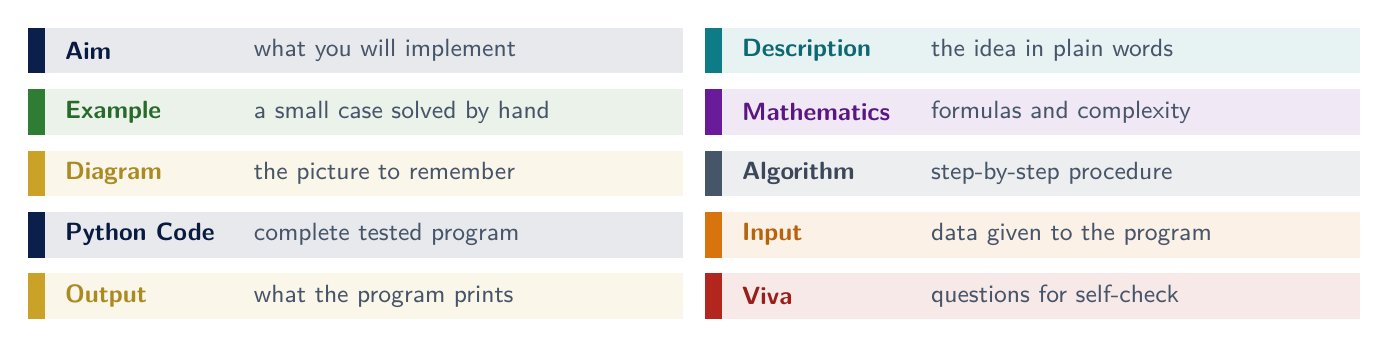
\begin{tikzpicture}[x=1cm,y=1cm]
  \foreach \name/\col/\txt [count=\i from 0] in {
     Aim/navy/what you will implement,
     Description/teal/the idea in plain words,
     Example/dgreen/a small case solved by hand,
     Mathematics/purple/formulas and complexity,
     Diagram/gold/the picture to remember,
     Algorithm/slate/step-by-step procedure,
     Python Code/navy/complete tested program,
     Input/orange/data given to the program,
     Output/gold/what the program prints,
     Viva/crimson/questions for self-check}{
    \pgfmathtruncatemacro{\r}{\i/2}
    \pgfmathtruncatemacro{\c}{\i-2*\r}
    \fill[\col] (\c*8.6,-\r*0.78) rectangle ++(0.22,0.58);
    \fill[\col!10] (\c*8.6+0.22,-\r*0.78) rectangle ++(8.1,0.58);
    \node[anchor=west,font=\sffamily\bfseries\small,text=\col!85!black] at (\c*8.6+0.35,-\r*0.78+0.29) {\name};
    \node[anchor=west,font=\sffamily\small,text=slate] at (\c*8.6+2.75,-\r*0.78+0.29) {\txt};}
\end{tikzpicture}

\clearpage
\markright{List of Experiments}
{\sffamily\bfseries\Large\color{navy}List of Experiments}\par
{\color{gold}\rule{\textwidth}{1.2pt}}

\renewcommand{\arraystretch}{1.5}
{\small
\begin{tabularx}{\textwidth}{>{\centering\arraybackslash\sffamily\bfseries}p{0.8cm}X>{\centering\arraybackslash}p{1.5cm}>{\centering\arraybackslash}p{0.9cm}>{\centering\arraybackslash}p{1.5cm}>{\centering\arraybackslash}p{1.1cm}>{\centering\arraybackslash}p{1.5cm}}
\rowcolor{navy}\textcolor{white}{No.} & \textcolor{white}{\sffamily\bfseries Laboratory Experiment / Practical Title} & \textcolor{white}{\sffamily\bfseries CO} & \textcolor{white}{\sffamily\bfseries Page} & \textcolor{white}{\sffamily\bfseries Date} & \textcolor{white}{\sffamily\bfseries Marks} & \textcolor{white}{\sffamily\bfseries Sign}\\
1 & Implement uninformed search (BFS and DFS) to solve the Water-Jug / 8-puzzle problem. & CO204.1 & \pageref{exp:1} & & & \\
\rowcolor{navy!8} 2 & Implement A* search with an admissible heuristic for the 8-puzzle or shortest-route problem. & CO204.2 & \pageref{exp:2} & & & \\
3 & Implement Hill Climbing / Best-First Search for a state-space problem. & CO204.2 & \pageref{exp:3} & & & \\
\rowcolor{navy!8} 4 & Implement game playing using the Minimax algorithm with Alpha-Beta pruning (e.g., Tic-Tac-Toe). & CO204.2 & \pageref{exp:4} & & & \\
5 & Solve a Constraint Satisfaction Problem (N-Queens / Map Colouring / Sudoku) using backtracking. & CO204.2 & \pageref{exp:5} & & & \\
\rowcolor{navy!8} 6 & Write a program (Prolog / Python) to represent facts and rules and answer queries using logical inference. & CO204.3 & \pageref{exp:6} & & & \\
7 & Implement unification and resolution for first-order logic statements. & CO204.3 & \pageref{exp:7} & & & \\
\rowcolor{navy!8} 8 & Implement Bayes' theorem / a simple Bayesian network for a diagnostic reasoning problem. & CO204.4 & \pageref{exp:8} & & & \\
9 & Build a decision-tree classifier on a small dataset and interpret the rules learned. & CO204.5 & \pageref{exp:9} & & & \\
\rowcolor{navy!8} 10 & Develop a simple rule-based expert system or a basic chatbot (mini-project). & CO204.5 & \pageref{exp:10} & & & \\
\end{tabularx}}

\vspace{10pt}
{\sffamily\bfseries\large\color{navy}Roadmap of the Laboratory}\par\vspace{4pt}
\begin{center}

\begin{tikzpicture}[x=1cm,y=1cm]
  \foreach \t/\e/\col [count=\i from 0] in {Search/Exp. 1--3/navy,Games/Exp. 4/teal,Constraints/Exp. 5/dgreen,Logic/Exp. 6--7/purple,Uncertainty/Exp. 8/orange,Learning \& ES/Exp. 9--10/crimson}{
    \node[fill=\col,text=white,rounded corners=4pt,minimum width=2.55cm,minimum height=1.25cm,align=center,font=\sffamily\bfseries\small] (n\i) at (\i*2.85,0) {\t\\[-1pt]{\normalfont\footnotesize \e}};}
  \foreach \i/\j in {0/1,1/2,2/3,3/4,4/5} \draw[-{Stealth[length=2mm]},gold,line width=1.4pt] (n\i)--(n\j);
\end{tikzpicture}
\end{center}

\vspace{6pt}
{\sffamily\bfseries\large\color{navy}General Instructions}\par
\begin{secbox}{BEFORE, DURING AND AFTER EACH SESSION}{navy}
\begin{enumerate}
  \item Read the Aim, Description and Mathematics of the experiment before coming to the laboratory.
  \item Solve the worked example by hand first; a program is easy to debug only when you know the expected answer.
  \item Type the program yourself, save it with the file name shown on the code box, and run it with \texttt{python filename.py}.
  \item Compare your output with the Output box. Then change the input (see the Input box) and explain the new output.
  \item Record the aim, algorithm, program, input and output in your journal and prepare the viva questions.
\end{enumerate}
\end{secbox}
% ============================ EXPERIMENT 1 ===========================
\experiment{Uninformed Search: Breadth-First Search and Depth-First Search for the Water-Jug Problem}{CO204.1}{BFS and DFS}

\begin{aim}
To formulate the Water-Jug problem as a state-space search problem and to solve it using the uninformed search strategies Breadth-First Search (BFS) and Depth-First Search (DFS).
\end{aim}

\begin{descr}
Two jugs of capacity 4 litres (A) and 3 litres (B) have no markings. Using a tap, we must obtain exactly 2 litres in jug A. A \textbf{state} is the pair $(a,b)$ of water currently in the jugs. Uninformed (blind) search uses no knowledge about how far a state is from the goal; it only knows how to generate successors and how to test for the goal.
\begin{itemize}
  \item \textbf{BFS} expands the shallowest node first using a FIFO \emph{queue}. It always finds a solution with the fewest moves.
  \item \textbf{DFS} expands the deepest node first using a LIFO \emph{stack}. It needs little memory but the solution found need not be the shortest.
\end{itemize}
Six operators are available: fill A, fill B, empty A, empty B, pour A into B, pour B into A.
\end{descr}

\begin{diagram}{state space of the Water-Jug problem}
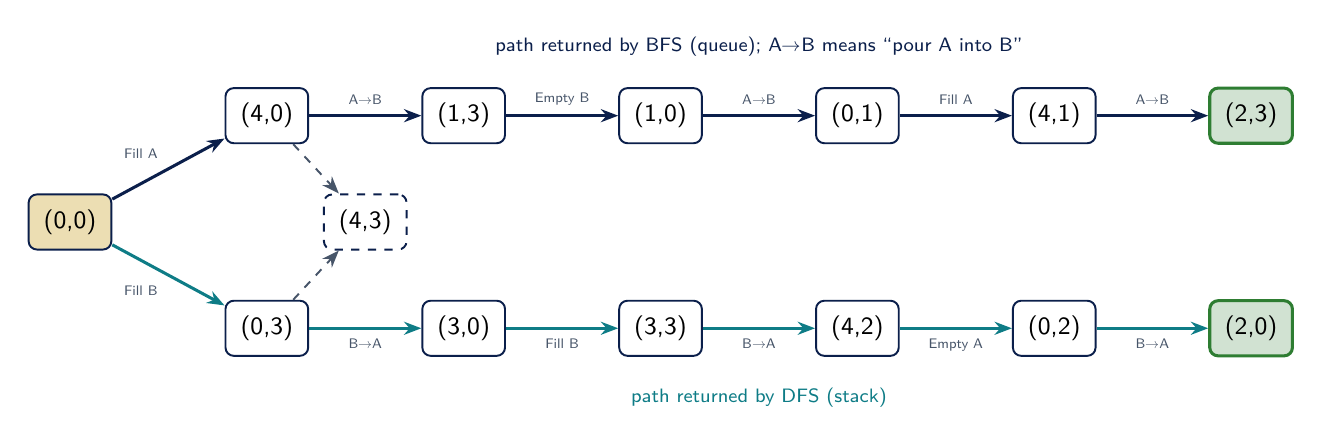
\begin{tikzpicture}[x=2.5cm,y=1.35cm,st/.append style={minimum width=10.5mm,inner xsep=2pt},lbl/.append style={font=\sffamily\tiny}]
  \node[st,fill=gold!35] (s) at (0,0) {(0,0)};
  \foreach \n/\x/\t in {a1/1/{(4,0)},a2/2/{(1,3)},a3/3/{(1,0)},a4/4/{(0,1)},a5/5/{(4,1)}} \node[st] (\n) at (\x,1) {\t};
  \node[goal] (a6) at (6,1) {(2,3)};
  \foreach \n/\x/\t in {b1/1/{(0,3)},b2/2/{(3,0)},b3/3/{(3,3)},b4/4/{(4,2)},b5/5/{(0,2)}} \node[st] (\n) at (\x,-1) {\t};
  \node[goal] (b6) at (6,-1) {(2,0)};
  \node[st,dashed] (m) at (1.5,0) {(4,3)};
  \draw[arr,navy,line width=1.1pt] (s) -- node[lbl,above left]{Fill A} (a1);
  \foreach \p/\q/\t in {a1/a2/A$\to$B,a2/a3/Empty B,a3/a4/A$\to$B,a4/a5/Fill A,a5/a6/A$\to$B}
    \draw[arr,navy,line width=1.1pt] (\p) -- node[lbl,above]{\t} (\q);
  \draw[arr,teal,line width=1.1pt] (s) -- node[lbl,below left]{Fill B} (b1);
  \foreach \p/\q/\t in {b1/b2/B$\to$A,b2/b3/Fill B,b3/b4/B$\to$A,b4/b5/Empty A,b5/b6/B$\to$A}
    \draw[arr,teal,line width=1.1pt] (\p) -- node[lbl,below]{\t} (\q);
  \draw[arr,dashed] (a1) -- (m); \draw[arr,dashed] (b1) -- (m);
  \node[lbl,text=navy,font=\sffamily\scriptsize] at (3.5,1.65) {path returned by BFS (queue); A$\to$B means ``pour A into B''};
  \node[lbl,text=teal,font=\sffamily\scriptsize] at (3.5,-1.65) {path returned by DFS (stack)};
\end{tikzpicture}

\vspace{4pt}

\begin{tikzpicture}[x=1cm,y=1cm]
  \node[lbl,text=navy,anchor=east] at (0,0) {\textbf{BFS frontier = QUEUE}};
  \foreach \i/\t in {0/A,1/B,2/C,3/D} \node[draw=navy,fill=navy!8,minimum size=6mm,font=\sffamily\scriptsize] at (0.5+\i*0.62,0) {\t};
  \node[lbl,anchor=west] at (2.75,0) {$\leftarrow$ in};
  \node[lbl] at (0.5,0.6) {out (oldest) $\downarrow$};
  \node[lbl,text=teal,anchor=east] at (8.6,0) {\textbf{DFS frontier = STACK}};
  \foreach \i/\t in {0/A,1/B,2/C,3/D} \node[draw=teal,fill=teal!8,minimum size=6mm,font=\sffamily\scriptsize] at (9.1+\i*0.62,0) {\t};
  \node[lbl] at (10.96,0.6) {$\downarrow$ in / out (newest)};
\end{tikzpicture}
\end{diagram}

\begin{example}
Start $(0,0)$. Applying the operators along the upper path of the diagram:
\[(0,0)\xrightarrow{\text{Fill A}}(4,0)\xrightarrow{\text{A}\to\text{B}}(1,3)\xrightarrow{\text{Empty B}}(1,0)\xrightarrow{\text{A}\to\text{B}}(0,1)\xrightarrow{\text{Fill A}}(4,1)\xrightarrow{\text{A}\to\text{B}}(2,3)\]
Jug A now holds exactly 2 litres after 6 moves. No shorter sequence exists, which BFS guarantees.
\end{example}

\begin{maths}
A search problem is the tuple $\langle S, s_0, A, T, G\rangle$ with states $S=\{(a,b)\mid 0\le a\le 4,\;0\le b\le 3\}$, so $|S| = 5\times 4 = 20$; initial state $s_0=(0,0)$; goal set $G=\{(2,b)\}$; unit step cost.

\textbf{Pour operator.} Pouring A into B moves $t=\min(a,\,3-b)$ litres: $(a,b)\mapsto(a-t,\;b+t)$.

\textbf{Solvability.} A target $d$ can be measured with jugs of capacity $m$ and $n$ if and only if
\[ d \le \max(m,n)\quad\text{and}\quad \gcd(m,n)\mid d . \]
Here $\gcd(4,3)=1$ divides 2, so a solution exists.

\textbf{Complexity} (branching factor $b$, shallowest goal depth $d$, maximum depth $m$):
\begin{center}\small
\begin{tabular}{lcccc}
\toprule
Strategy & Complete & Optimal (unit cost) & Time & Space\\ \midrule
BFS & Yes & Yes & $O(b^{d})$ & $O(b^{d})$\\
DFS (graph search, finite space) & Yes & No & $O(b^{m})$ & $O(bm)$\\
\bottomrule
\end{tabular}
\end{center}
\end{maths}

\begin{algorithm}
\begin{enumerate}
  \item Put the start state in the frontier and record it as visited.
  \item Remove a state from the frontier: from the \emph{front} for BFS, from the \emph{back} for DFS.
  \item If it is a goal state, follow the parent links backwards and return the path.
  \item Otherwise generate all successors; add each unvisited successor to the frontier and store its parent.
  \item Repeat steps 2 to 4 until the frontier is empty (then no solution exists).
\end{enumerate}
\end{algorithm}

\begin{pycode}{exp01\_bfs\_dfs\_water\_jug.py}
"""Experiment 1: Uninformed Search (BFS and DFS) - Water Jug Problem."""
from collections import deque

CAP_A, CAP_B, TARGET = 4, 3, 2       # jug capacities and goal amount


def successors(state):
    """Return every (next_state, action) reachable from 'state'."""
    a, b = state
    pour_ab = min(a, CAP_B - b)      # litres that can move A -> B
    pour_ba = min(b, CAP_A - a)      # litres that can move B -> A
    moves = [
        ((CAP_A, b), "Fill jug A"),
        ((a, CAP_B), "Fill jug B"),
        ((0, b), "Empty jug A"),
        ((a, 0), "Empty jug B"),
        ((a - pour_ab, b + pour_ab), "Pour A -> B"),
        ((a + pour_ba, b - pour_ba), "Pour B -> A"),
    ]
    return [(s, act) for s, act in moves if s != state]


def is_goal(state):
    return state[0] == TARGET


def build_path(parent, state):
    """Walk back through the parent links to recover the solution."""
    path = []
    while parent[state] is not None:
        previous, action = parent[state]
        path.append((action, state))
        state = previous
    return path[::-1]


def search(start, strategy):
    """Generic graph search. BFS uses a FIFO queue, DFS a LIFO stack."""
    frontier = deque([start])
    parent = {start: None}           # also acts as the visited set
    expanded = 0
    while frontier:
        state = frontier.popleft() if strategy == "BFS" else frontier.pop()
        expanded += 1
        if is_goal(state):
            return build_path(parent, state), expanded
        for nxt, action in successors(state):
            if nxt not in parent:
                parent[nxt] = (state, action)
                frontier.append(nxt)
    return None, expanded


def report(strategy, start):
    path, expanded = search(start, strategy)
    print(f"\n===== {strategy} =====")
    if path is None:
        print("No solution exists.")
        return
    print(f"Step  0: {'Start':<13} -> {start}")
    for i, (action, state) in enumerate(path, 1):
        print(f"Step {i:2d}: {action:<13} -> {state}")
    print(f"Solution length : {len(path)} moves")
    print(f"Nodes expanded  : {expanded}")


if __name__ == "__main__":
    print(f"Water Jug Problem: A = {CAP_A} L, B = {CAP_B} L, "
          f"goal = {TARGET} L in jug A")
    for name in ("BFS", "DFS"):
        report(name, (0, 0))
\end{pycode}

\begin{inputbox}
The input is set at the top of the program: \texttt{CAP\_A = 4}, \texttt{CAP\_B = 3}, \texttt{TARGET = 2}, start state \texttt{(0, 0)}. Try \texttt{CAP\_A, CAP\_B, TARGET = 5, 3, 4} and \texttt{6, 4, 3} (the second has no solution because $\gcd(6,4)=2$ does not divide 3).
\end{inputbox}

\begin{outputbox}
Water Jug Problem: A = 4 L, B = 3 L, goal = 2 L in jug A

===== BFS =====
Step  0: Start         -> (0, 0)
Step  1: Fill jug A    -> (4, 0)
Step  2: Pour A -> B   -> (1, 3)
Step  3: Empty jug B   -> (1, 0)
Step  4: Pour A -> B   -> (0, 1)
Step  5: Fill jug A    -> (4, 1)
Step  6: Pour A -> B   -> (2, 3)
Solution length : 6 moves
Nodes expanded  : 13

===== DFS =====
Step  0: Start         -> (0, 0)
Step  1: Fill jug B    -> (0, 3)
Step  2: Pour B -> A   -> (3, 0)
Step  3: Fill jug B    -> (3, 3)
Step  4: Pour B -> A   -> (4, 2)
Step  5: Empty jug A   -> (0, 2)
Step  6: Pour B -> A   -> (2, 0)
Solution length : 6 moves
Nodes expanded  : 7
\end{outputbox}

\begin{result}
The Water-Jug problem was modelled as a state space and solved by BFS and DFS. BFS returned a shortest solution of 6 moves; DFS also reached a goal but explored the space in a different order.
\end{result}

\begin{viva}
\begin{enumerate}
  \item Why is BFS optimal only when all step costs are equal?
  \item Which data structure turns the same code from BFS into DFS?
  \item What is the purpose of the visited set? What happens to DFS without it?
  \item How does Iterative Deepening combine the advantages of BFS and DFS?
  \item State the condition under which a water-jug target cannot be measured.
\end{enumerate}
\end{viva}

% ============================ EXPERIMENT 2 ===========================
\experiment{A* Search with an Admissible Heuristic for the 8-Puzzle Problem}{CO204.2}{A* Search}

\begin{aim}
To implement the A* algorithm for the 8-puzzle using the admissible heuristics ``misplaced tiles'' and ``Manhattan distance'', and to compare the number of nodes they expand.
\end{aim}

\begin{descr}
The 8-puzzle has eight numbered tiles and one blank on a $3\times 3$ board. A move slides the blank up, down, left or right. A* is an \textbf{informed} search: it ranks every node $n$ by
$f(n)=g(n)+h(n)$, where $g(n)$ is the cost already paid from the start and $h(n)$ is an \emph{estimate} of the cost still to pay. The node with the smallest $f$ is expanded first (priority queue). If $h$ never overestimates, the first time the goal is removed from the queue the path found is optimal.
\end{descr}

\begin{diagram}{first expansion of A* (Manhattan heuristic)}
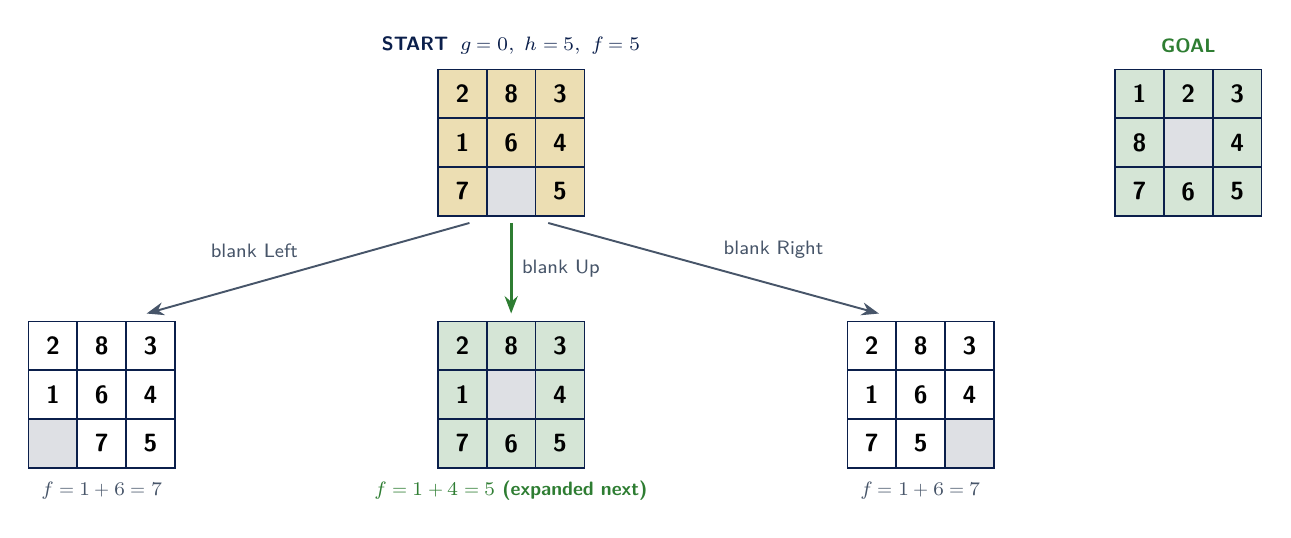
\begin{tikzpicture}[x=1cm,y=1cm]
  \puzzle{5.6}{0}{2,8,3,1,6,4,7,0,5}{gold!35}
  \node[lbl,text=navy] at (6.53,0.3) {\textbf{START}\; $g=0,\ h=5,\ f=5$};
  \puzzle{0.4}{-3.2}{2,8,3,1,6,4,0,7,5}{white}
  \puzzle{5.6}{-3.2}{2,8,3,1,0,4,7,6,5}{dgreen!20}
  \puzzle{10.8}{-3.2}{2,8,3,1,6,4,7,5,0}{white}
  \draw[arr] (6.0,-1.95) -- node[lbl,above left]{blank Left} (1.9,-3.1);
  \draw[arr,dgreen,line width=1.2pt] (6.53,-1.95) -- node[lbl,right]{blank Up} (6.53,-3.1);
  \draw[arr] (7.0,-1.95) -- node[lbl,above right]{blank Right} (11.2,-3.1);
  \node[lbl] at (1.33,-5.35) {$f = 1+6 = 7$};
  \node[lbl,text=dgreen] at (6.53,-5.35) {$f = 1+4 = 5$ \textbf{(expanded next)}};
  \node[lbl] at (11.73,-5.35) {$f = 1+6 = 7$};
  \puzzle{14.2}{0}{1,2,3,8,0,4,7,6,5}{dgreen!20}
  \node[lbl,text=dgreen] at (15.13,0.3) {\textbf{GOAL}};
\end{tikzpicture}
\end{diagram}

\begin{example}
For the start state, the Manhattan distance is obtained tile by tile: tile 2 is 1 step from its goal cell, tile 8 is 2 steps, tile 1 is 1 step and tile 6 is 1 step; tiles 3, 4, 5, 7 are in place. Hence $h_2 = 1+2+1+1 = 5$. Four tiles (1, 2, 6, 8) are misplaced, so $h_1 = 4$. A* expands the child with $f=5$ and continues until $h=0$; the optimal solution has 5 moves: Up, Up, Left, Down, Right.
\end{example}

\begin{maths}
\textbf{Evaluation function:}\quad $f(n) = g(n) + h(n)$.

\textbf{Admissible:}\quad $0 \le h(n) \le h^{*}(n)$ for every $n$, where $h^{*}(n)$ is the true cheapest cost from $n$ to a goal.

\textbf{Consistent (monotone):}\quad $h(n) \le c(n,a,n') + h(n')$ for every successor $n'$ of $n$. Consistency implies admissibility and makes $f$ non-decreasing along any path.

\textbf{Heuristics for the 8-puzzle:}
\[ h_1(n) = \sum_{t=1}^{8} [\,\text{tile } t \text{ is not in its goal cell}\,], \qquad
   h_2(n) = \sum_{t=1}^{8} \bigl(|r_t - r_t^{g}| + |c_t - c_t^{g}|\bigr). \]
Both are admissible because every move shifts one tile by one cell. Since $h_1(n)\le h_2(n)\le h^{*}(n)$, $h_2$ \emph{dominates} $h_1$ and A* with $h_2$ never expands more nodes than with $h_1$ (apart from ties).

\textbf{Solvability:} let $\mathrm{inv}(s)$ be the number of pairs of tiles that appear in reverse order when the board is read row by row (blank ignored). On a $3\times3$ board a state can reach the goal iff $\mathrm{inv}(s)\equiv \mathrm{inv}(goal) \pmod 2$. Here $\mathrm{inv}(start)=11$ and $\mathrm{inv}(goal)=7$, both odd. Exactly $9!/2 = 181{,}440$ states are reachable.
\end{maths}

\begin{algorithm}
\begin{enumerate}
  \item Insert the start node into the priority queue OPEN with $f = h(start)$; set $g(start)=0$.
  \item Remove from OPEN the node $n$ with the smallest $f$. If $n$ is the goal, rebuild and return the path.
  \item For every successor $n'$ of $n$ compute $g' = g(n) + 1$.
  \item If $n'$ is new, or $g'$ is smaller than the best known $g(n')$, store $g(n') = g'$, remember $n$ as its parent and push $n'$ with priority $g' + h(n')$.
  \item Repeat from step 2 until OPEN is empty.
\end{enumerate}
\end{algorithm}

\begin{pycode}{exp02\_astar\_8puzzle.py}
"""Experiment 2: A* Search with admissible heuristics - 8-Puzzle."""
import heapq

GOAL = (1, 2, 3,
        8, 0, 4,
        7, 6, 5)                      # 0 denotes the blank tile
GOAL_POS = {tile: divmod(i, 3) for i, tile in enumerate(GOAL)}


def h_misplaced(state):
    """h1: number of tiles that are not in their goal cell."""
    return sum(1 for i, t in enumerate(state) if t != 0 and t != GOAL[i])


def h_manhattan(state):
    """h2: sum of horizontal + vertical distances of tiles from goal."""
    total = 0
    for i, tile in enumerate(state):
        if tile != 0:
            r, c = divmod(i, 3)
            gr, gc = GOAL_POS[tile]
            total += abs(r - gr) + abs(c - gc)
    return total


def neighbours(state):
    """Slide the blank Up, Down, Left or Right (each move costs 1)."""
    z = state.index(0)
    r, c = divmod(z, 3)
    for dr, dc, name in ((-1, 0, "Up"), (1, 0, "Down"),
                         (0, -1, "Left"), (0, 1, "Right")):
        nr, nc = r + dr, c + dc
        if 0 <= nr < 3 and 0 <= nc < 3:
            s = list(state)
            s[z], s[nr * 3 + nc] = s[nr * 3 + nc], s[z]
            yield tuple(s), name


def inversions(state):
    tiles = [t for t in state if t != 0]
    return sum(tiles[i] > tiles[j]
               for i in range(len(tiles)) for j in range(i + 1, len(tiles)))


def solvable(start):
    """On a 3x3 board a state can reach GOAL iff parities match."""
    return inversions(start) % 2 == inversions(GOAL) % 2


def astar(start, h):
    open_list = [(h(start), 0, start)]          # entries are (f, g, state)
    g_cost = {start: 0}
    parent = {start: None}
    expanded = 0
    while open_list:
        f, g, state = heapq.heappop(open_list)
        if g > g_cost[state]:
            continue                            # stale queue entry
        expanded += 1
        if state == GOAL:
            path = []
            while parent[state] is not None:
                state, move = parent[state][0], parent[state][1]
                path.append(move)
            return path[::-1], expanded
        for nxt, move in neighbours(state):
            new_g = g + 1
            if new_g < g_cost.get(nxt, float("inf")):
                g_cost[nxt] = new_g
                parent[nxt] = (state, move)
                heapq.heappush(open_list, (new_g + h(nxt), new_g, nxt))
    return None, expanded


def show(state):
    for r in range(3):
        print("   " + " ".join("_" if t == 0 else str(t)
                               for t in state[3 * r:3 * r + 3]))


def apply(state, move):
    return next(s for s, m in neighbours(state) if m == move)


if __name__ == "__main__":
    start = (2, 8, 3,
             1, 6, 4,
             7, 0, 5)
    print("Solvable:", solvable(start))
    path, expanded = astar(start, h_manhattan)
    state = start
    print(f"g=0 h={h_manhattan(state)} f={h_manhattan(state)}  (start)")
    show(state)
    for g, move in enumerate(path, 1):
        state = apply(state, move)
        h = h_manhattan(state)
        print(f"g={g} h={h} f={g + h}  (blank moved {move})")
        show(state)
    print("Optimal moves :", " -> ".join(path))
    print("Path cost     :", len(path))

    hard = (2, 1, 6,
            4, 0, 8,
            7, 5, 3)
    print("\nHeuristic comparison on a harder instance", hard)
    for name, h in (("h1 misplaced", h_misplaced), ("h2 Manhattan", h_manhattan)):
        p, n = astar(hard, h)
        print(f"  {name:<13}: cost = {len(p):2d}, nodes expanded = {n}")
\end{pycode}

\begin{inputbox}
Start state \texttt{(2,8,3, 1,6,4, 7,0,5)} and goal \texttt{(1,2,3, 8,0,4, 7,6,5)}, where \texttt{0} is the blank. A second, harder start state \texttt{(2,1,6, 4,0,8, 7,5,3)} is used to compare the two heuristics.
\end{inputbox}

\begin{outputbox}
Solvable: True
g=0 h=5 f=5  (start)
   2 8 3
   1 6 4
   7 _ 5
g=1 h=4 f=5  (blank moved Up)
   2 8 3
   1 _ 4
   7 6 5
g=2 h=3 f=5  (blank moved Up)
   2 _ 3
   1 8 4
   7 6 5
g=3 h=2 f=5  (blank moved Left)
   _ 2 3
   1 8 4
   7 6 5
g=4 h=1 f=5  (blank moved Down)
   1 2 3
   _ 8 4
   7 6 5
g=5 h=0 f=5  (blank moved Right)
   1 2 3
   8 _ 4
   7 6 5
Optimal moves : Up -> Up -> Left -> Down -> Right
Path cost     : 5

Heuristic comparison on a harder instance (2, 1, 6, 4, 0, 8, 7, 5, 3)
  h1 misplaced : cost = 18, nodes expanded = 1747
  h2 Manhattan : cost = 18, nodes expanded = 229
\end{outputbox}

\begin{result}
A* found the optimal 5-move solution. On the harder instance both heuristics returned the same optimal cost (18), but Manhattan distance expanded far fewer nodes than misplaced tiles, confirming that a more informed admissible heuristic reduces search effort.
\end{result}

\begin{viva}
\begin{enumerate}
  \item What happens to A* when $h(n)=0$ for all $n$? Which algorithm does it become?
  \item Give an example of a heuristic for the 8-puzzle that is \emph{not} admissible.
  \item Why does a dominating heuristic expand fewer nodes?
  \item Distinguish between admissibility and consistency.
  \item Why is the memory requirement the main drawback of A*?
\end{enumerate}
\end{viva}

% ============================ EXPERIMENT 3 ===========================
\experiment{Hill Climbing and Best-First Search for a State-Space Problem}{CO204.2}{Hill Climbing / Best-First}

\begin{aim}
To implement (a) steepest-ascent Hill Climbing with random restart for the 8-Queens problem and (b) Greedy Best-First Search for route finding on the Romania road map.
\end{aim}

\begin{descr}
\textbf{Hill climbing} is a local search: it keeps only the current state and repeatedly moves to the best neighbouring state. It stops when no neighbour is better. It is fast and uses constant memory, but it can stop at a local optimum, on a plateau or on a ridge. \textbf{Random restart} overcomes this by starting again from a new random state.

\textbf{Greedy best-first search} keeps a frontier but always expands the node that \emph{appears} closest to the goal, i.e. the one with the smallest heuristic $h(n)$, ignoring the cost already paid. It is usually quick but is neither optimal nor complete in general.
\end{descr}

\begin{diagram}{state-space landscape seen by hill climbing}
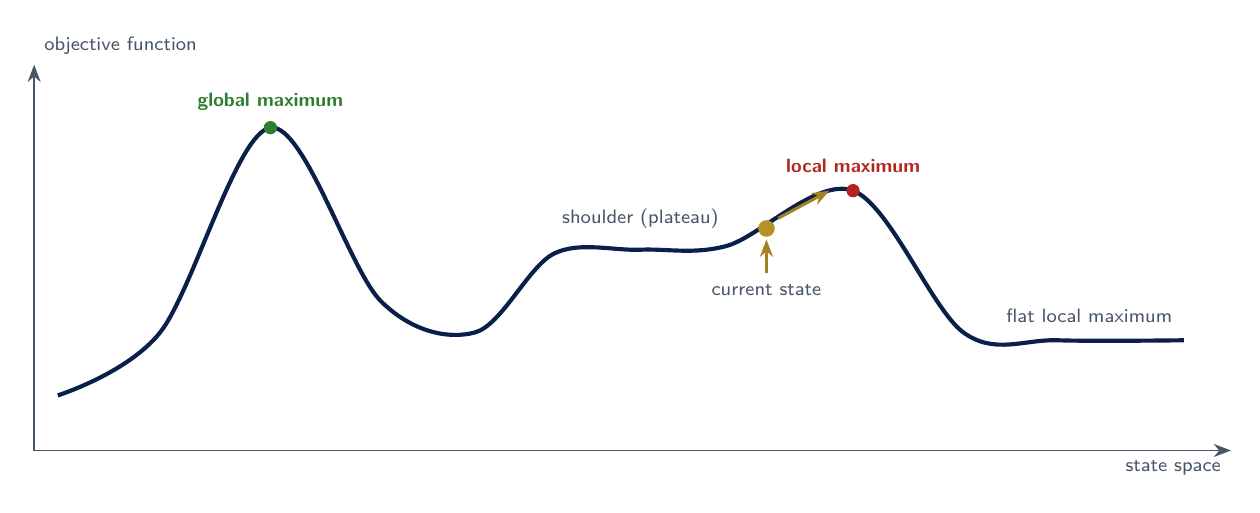
\begin{tikzpicture}[x=1cm,y=1cm]
  \draw[arr] (0,0) -- (15.2,0) node[lbl,below left] {state space};
  \draw[arr] (0,0) -- (0,4.9) node[lbl,above right] {objective function};
  \draw[navy,line width=1.5pt] plot[smooth,tension=0.55] coordinates {(0.3,0.7) (1.6,1.5) (3.0,4.1) (4.4,1.9) (5.6,1.5) (6.6,2.5) (7.7,2.55) (8.8,2.6) (10.4,3.3) (11.8,1.5) (13.0,1.4) (14.6,1.4)};
  \fill[dgreen] (3.0,4.1) circle (2.4pt); \node[lbl,text=dgreen,above] at (3.0,4.2) {\textbf{global maximum}};
  \fill[crimson] (10.4,3.3) circle (2.4pt); \node[lbl,text=crimson,above] at (10.4,3.4) {\textbf{local maximum}};
  \node[lbl,above] at (7.7,2.7) {shoulder (plateau)};
  \node[lbl,above] at (13.4,1.5) {flat local maximum};
  \fill[gold!90!black] (9.3,2.82) circle (3pt);
  \draw[arr,gold!80!black,line width=1.1pt] (9.3,2.25) node[lbl,below]{current state} -- (9.3,2.68);
  \draw[arr,gold!80!black,line width=1.1pt] (9.45,2.95) -- (10.1,3.3);
\end{tikzpicture}
\end{diagram}

\begin{example}
\textbf{8-Queens.} A state is $(r_1,\dots,r_8)$ where $r_c$ is the row of the queen in column $c$. For the state $(2,4,1,7,0,6,3,5)$ no two queens share a row or a diagonal, so $h=0$ (a solution). Each state has $8\times 7 = 56$ neighbours (move one queen within its column).

\textbf{Greedy best-first.} From Arad the successors are Sibiu ($h=253$), Timisoara ($h=329$) and Zerind ($h=374$). Sibiu is chosen, then Fagaras ($h=176$), then Bucharest: path cost $140+99+211=450$ km. The cheaper route through Rimnicu and Pitesti (418 km) is missed because greedy search ignores $g(n)$.
\end{example}

\begin{maths}
\textbf{Hill-climbing update:}\quad $s_{t+1} = \arg\min_{s'\in N(s_t)} h(s')$, stop when $h(s_{t+1}) \ge h(s_t)$.

\textbf{Objective for $N$-Queens:} number of attacking pairs
\[ h(s) = \bigl|\{(i,j)\;:\; i<j,\ r_i = r_j \ \text{or}\ |r_i-r_j| = j-i\}\bigr|, \qquad 0\le h(s)\le \tbinom{8}{2}=28 . \]

\textbf{Random restart:} if one run succeeds with probability $p$, the expected number of runs is $1/p$. For 8-Queens steepest ascent succeeds for about $14\%$ of random starts, so roughly $1/0.14\approx 7$ restarts are needed on average.

\textbf{Greedy best-first:}\quad $f(n) = h(n)$\quad (compare with A*: $f(n)=g(n)+h(n)$). Worst-case time and space are $O(b^{m})$.
\end{maths}

\begin{algorithm}
\textbf{Hill climbing with random restart}
\begin{enumerate}
  \item Generate a random state and compute $h$.
  \item Evaluate all neighbours; move to the neighbour with the lowest $h$ if it is better than the current state.
  \item If no neighbour is better, stop this run: if $h=0$ report the solution, otherwise restart from step 1.
\end{enumerate}
\textbf{Greedy best-first search}
\begin{enumerate}
  \item Push the start node into a priority queue ordered by $h$.
  \item Pop the node with the smallest $h$; if it is the goal, return the path.
  \item Push all unvisited successors with their $h$ values and repeat.
\end{enumerate}
\end{algorithm}

\begin{pycode}{exp03\_hill\_climbing\_best\_first.py}
"""Experiment 3: Hill Climbing (8-Queens) and Greedy Best-First Search."""
import heapq
import random

N = 8


# ---------- Part A: steepest-ascent hill climbing with random restart ------
def conflicts(state):
    """h(n): number of pairs of queens attacking each other.
    state[c] = row of the queen placed in column c."""
    return sum(1 for a in range(N) for b in range(a + 1, N)
               if state[a] == state[b] or abs(state[a] - state[b]) == b - a)


def best_neighbour(state):
    """Move one queen inside its column; return the lowest-h neighbour."""
    best, best_h = state, conflicts(state)
    for col in range(N):
        for row in range(N):
            if row != state[col]:
                cand = state[:col] + (row,) + state[col + 1:]
                h = conflicts(cand)
                if h < best_h:
                    best, best_h = cand, h
    return best, best_h


def hill_climb(state):
    steps = 0
    while True:
        nxt, h = best_neighbour(state)
        if nxt == state:                 # no better neighbour: peak reached
            return state, conflicts(state), steps
        state, steps = nxt, steps + 1


def random_restart(seed=7, max_restarts=50):
    rng = random.Random(seed)
    for attempt in range(1, max_restarts + 1):
        start = tuple(rng.randrange(N) for _ in range(N))
        final, h, steps = hill_climb(start)
        status = "GLOBAL optimum" if h == 0 else "stuck (local optimum)"
        print(f"Restart {attempt}: start h = {conflicts(start):2d} -> "
              f"final h = {h} after {steps} steps  [{status}]")
        if h == 0:
            return final
    return None


def show_board(state):
    for row in range(N):
        print("   " + " ".join("Q" if state[c] == row else "." for c in range(N)))


# ---------- Part B: greedy best-first search on the Romania road map -------
GRAPH = {
    "Arad": {"Zerind": 75, "Sibiu": 140, "Timisoara": 118},
    "Zerind": {"Arad": 75, "Oradea": 71},
    "Oradea": {"Zerind": 71, "Sibiu": 151},
    "Timisoara": {"Arad": 118, "Lugoj": 111},
    "Lugoj": {"Timisoara": 111, "Mehadia": 70},
    "Mehadia": {"Lugoj": 70, "Drobeta": 75},
    "Drobeta": {"Mehadia": 75, "Craiova": 120},
    "Sibiu": {"Arad": 140, "Oradea": 151, "Fagaras": 99, "Rimnicu": 80},
    "Fagaras": {"Sibiu": 99, "Bucharest": 211},
    "Rimnicu": {"Sibiu": 80, "Pitesti": 97, "Craiova": 146},
    "Craiova": {"Drobeta": 120, "Rimnicu": 146, "Pitesti": 138},
    "Pitesti": {"Rimnicu": 97, "Craiova": 138, "Bucharest": 101},
    "Bucharest": {"Fagaras": 211, "Pitesti": 101},
}
H_SLD = {"Arad": 366, "Zerind": 374, "Oradea": 380, "Timisoara": 329,
         "Lugoj": 244, "Mehadia": 241, "Drobeta": 242, "Sibiu": 253,
         "Fagaras": 176, "Rimnicu": 193, "Craiova": 160, "Pitesti": 100,
         "Bucharest": 0}


def greedy_best_first(start, goal):
    frontier = [(H_SLD[start], start)]           # ordered by h(n) only
    parent = {start: None}
    while frontier:
        h, city = heapq.heappop(frontier)
        print(f"   expand {city:<10} h = {h}")
        if city == goal:
            path = []
            while city is not None:
                path.append(city)
                city = parent[city]
            return path[::-1]
        for nxt in GRAPH[city]:
            if nxt not in parent:
                parent[nxt] = city
                heapq.heappush(frontier, (H_SLD[nxt], nxt))
    return None


if __name__ == "__main__":
    print("PART A: Hill climbing on the 8-Queens problem")
    solution = random_restart()
    print("Solution (row of queen in each column):", solution)
    show_board(solution)

    print("\nPART B: Greedy best-first search, Arad -> Bucharest")
    path = greedy_best_first("Arad", "Bucharest")
    cost = sum(GRAPH[a][b] for a, b in zip(path, path[1:]))
    print("Path :", " -> ".join(path))
    print("Cost :", cost, "km  (optimal is 418 km via Rimnicu and Pitesti)")
\end{pycode}

\begin{inputbox}
Part A: board size \texttt{N = 8}, random seed \texttt{7} (change the seed to see different restarts). Part B: the Romania road map \texttt{GRAPH}, straight-line distances to Bucharest \texttt{H\_SLD}, start \texttt{Arad}, goal \texttt{Bucharest}.
\end{inputbox}

\begin{outputbox}
PART A: Hill climbing on the 8-Queens problem
Restart 1: start h =  6 -> final h = 1 after 3 steps  [stuck (local optimum)]
Restart 2: start h =  9 -> final h = 1 after 3 steps  [stuck (local optimum)]
Restart 3: start h = 10 -> final h = 0 after 5 steps  [GLOBAL optimum]
Solution (row of queen in each column): (2, 4, 1, 7, 0, 6, 3, 5)
   . . . . Q . . .
   . . Q . . . . .
   Q . . . . . . .
   . . . . . . Q .
   . Q . . . . . .
   . . . . . . . Q
   . . . . . Q . .
   . . . Q . . . .

PART B: Greedy best-first search, Arad -> Bucharest
   expand Arad       h = 366
   expand Sibiu      h = 253
   expand Fagaras    h = 176
   expand Bucharest  h = 0
Path : Arad -> Sibiu -> Fagaras -> Bucharest
Cost : 450 km  (optimal is 418 km via Rimnicu and Pitesti)
\end{outputbox}

\begin{result}
Hill climbing became stuck at local optima in the first two runs and reached a conflict-free 8-Queens placement on the third restart. Greedy best-first search reached Bucharest after expanding only four nodes, but its 450 km route is longer than the optimal 418 km route.
\end{result}

\begin{viva}
\begin{enumerate}
  \item What are local maxima, plateaux and ridges?
  \item How does simulated annealing escape a local optimum?
  \item Why is hill climbing called a ``greedy local search''?
  \item Why is greedy best-first search not optimal? Give the Romania example.
  \item Compare stochastic hill climbing with steepest-ascent hill climbing.
\end{enumerate}
\end{viva}

% ============================ EXPERIMENT 4 ===========================
\experiment{Game Playing with the Minimax Algorithm and Alpha-Beta Pruning (Tic-Tac-Toe)}{CO204.2}{Minimax and Alpha-Beta}

\begin{aim}
To implement the Minimax algorithm and its Alpha-Beta pruned version for Tic-Tac-Toe, and to compare the number of game-tree nodes each one visits.
\end{aim}

\begin{descr}
Tic-Tac-Toe is a two-player, zero-sum, deterministic game with perfect information. Player X (MAX) tries to maximise the final score; player O (MIN) tries to minimise it. \textbf{Minimax} explores the complete game tree and assumes both players play perfectly. \textbf{Alpha-Beta pruning} returns exactly the same move but skips branches that cannot influence the decision. It keeps two bounds: $\alpha$, the best value MAX can already guarantee, and $\beta$, the best value MIN can already guarantee. When $\alpha\ge\beta$ the remaining children are pruned.
\end{descr}

\begin{diagram}{Alpha-Beta pruning on a two-ply game tree}
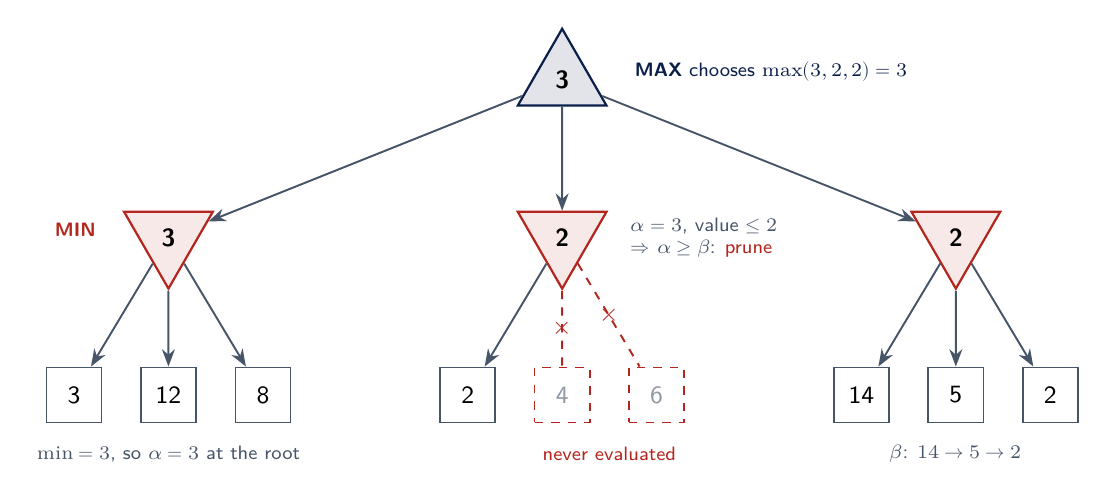
\begin{tikzpicture}[x=1cm,y=1cm]
  \node[maxn] (r) at (0,0) {3};
  \node[minn] (a) at (-5,-2) {3}; \node[minn] (b) at (0,-2) {2}; \node[minn] (c) at (5,-2) {2};
  \foreach \p/\x/\v in {a/-6.2/3,a/-5/12,a/-3.8/8,b/-1.2/2,c/3.8/14,c/5/5,c/6.2/2}{
    \node[leaf] (l\p\v) at (\x,-4) {\v}; \draw[arr] (\p) -- (l\p\v);}
  \foreach \x/\v in {0/4,1.2/6}{
    \node[leaf,dashed,draw=crimson,text=slate!60] (p\v) at (\x,-4) {\v};
    \draw[dashed,crimson,line width=0.7pt] (b) -- node[pos=0.5,font=\sffamily\bfseries\small,text=crimson]{$\times$} (p\v);}
  \draw[arr] (r) -- (a); \draw[arr] (r) -- (b); \draw[arr] (r) -- (c);
  \node[lbl,text=navy,anchor=west] at (0.8,0.1) {\textbf{MAX} chooses $\max(3,2,2)=3$};
  \node[lbl,text=crimson,anchor=east] at (-5.8,-1.9) {\textbf{MIN}};
  \node[lbl,anchor=west,align=left] at (0.75,-2.0) {$\alpha=3$, value $\le 2$\\ $\Rightarrow$ $\alpha\ge\beta$: \textcolor{crimson}{prune}};
  \node[lbl] at (-5,-4.75) {$\min = 3$, so $\alpha = 3$ at the root};
  \node[lbl,text=crimson] at (0.6,-4.75) {never evaluated};
  \node[lbl] at (5,-4.75) {$\beta$: $14 \to 5 \to 2$};
\end{tikzpicture}
\end{diagram}

\begin{example}
In the tree above the left MIN node returns $\min(3,12,8)=3$, so MAX is guaranteed at least $\alpha=3$. At the middle MIN node the first leaf is 2, so this node is worth at most 2, which is already worse for MAX than 3. Its other leaves (4 and 6) cannot change the decision and are pruned. The right MIN node returns 2. The root value is $\max(3,2,2)=3$ and only 7 of the 9 leaves were examined.
\end{example}

\begin{maths}
\textbf{Minimax value} of a state $s$:
\[ \mathrm{Minimax}(s)=\begin{cases}
\mathrm{Utility}(s) & \text{if } s \text{ is terminal}\\[2pt]
\max_{a\in \mathrm{Actions}(s)} \mathrm{Minimax}(\mathrm{Result}(s,a)) & \text{if MAX is to move}\\[2pt]
\min_{a\in \mathrm{Actions}(s)} \mathrm{Minimax}(\mathrm{Result}(s,a)) & \text{if MIN is to move}
\end{cases} \]
\textbf{Utility used in the program:} $U = 10-d$ if X wins, $d-10$ if O wins and $0$ for a draw, where $d$ is the depth of the terminal state (faster wins are preferred).

\textbf{Pruning rule:} at a MAX node update $\alpha=\max(\alpha,v)$; at a MIN node update $\beta=\min(\beta,v)$; stop examining children as soon as $\alpha\ge\beta$.

\textbf{Complexity} for branching factor $b$ and depth $m$: Minimax takes $O(b^{m})$ time; Alpha-Beta with perfect move ordering takes $O(b^{m/2})$, so it can search about twice as deep in the same time. For Tic-Tac-Toe the number of move sequences is at most $9! = 362{,}880$.
\end{maths}

\begin{algorithm}
\begin{enumerate}
  \item If the board is terminal (win, loss or draw) return its utility.
  \item If it is MAX's turn: set $v=-\infty$; for each empty cell place X, call the procedure recursively for MIN, undo the move, set $v=\max(v,\text{score})$ and $\alpha=\max(\alpha,v)$; if $\alpha\ge\beta$ stop the loop.
  \item If it is MIN's turn: set $v=+\infty$; for each empty cell place O, recurse for MAX, undo the move, set $v=\min(v,\text{score})$ and $\beta=\min(\beta,v)$; if $\alpha\ge\beta$ stop the loop.
  \item Return $v$ together with the move that produced it.
\end{enumerate}
\end{algorithm}

\begin{pycode}{exp04\_minimax\_alphabeta\_tictactoe.py}
"""Experiment 4: Minimax with Alpha-Beta pruning - Tic-Tac-Toe."""
import math

LINES = [(0, 1, 2), (3, 4, 5), (6, 7, 8),      # rows
         (0, 3, 6), (1, 4, 7), (2, 5, 8),      # columns
         (0, 4, 8), (2, 4, 6)]                 # diagonals
HUMAN_PLAYS = False        # set True to play as O against the computer
nodes = 0                  # counts the game-tree nodes visited


def winner(board):
    for a, b, c in LINES:
        if board[a] != " " and board[a] == board[b] == board[c]:
            return board[a]
    return "Draw" if " " not in board else None


def utility(result, depth):
    """+ve for X (MAX), -ve for O (MIN); quicker wins score higher."""
    if result == "X":
        return 10 - depth
    if result == "O":
        return depth - 10
    return 0


def minimax(board, player, depth=0):
    global nodes
    nodes += 1
    result = winner(board)
    if result:
        return utility(result, depth), None
    best_move = None
    best = -math.inf if player == "X" else math.inf
    for cell in range(9):
        if board[cell] == " ":
            board[cell] = player
            score, _ = minimax(board, "O" if player == "X" else "X", depth + 1)
            board[cell] = " "
            if (player == "X" and score > best) or \
               (player == "O" and score < best):
                best, best_move = score, cell
    return best, best_move


def alphabeta(board, player, depth=0, alpha=-math.inf, beta=math.inf):
    global nodes
    nodes += 1
    result = winner(board)
    if result:
        return utility(result, depth), None
    best_move = None
    if player == "X":                               # MAX node
        best = -math.inf
        for cell in range(9):
            if board[cell] == " ":
                board[cell] = "X"
                score, _ = alphabeta(board, "O", depth + 1, alpha, beta)
                board[cell] = " "
                if score > best:
                    best, best_move = score, cell
                alpha = max(alpha, best)
                if alpha >= beta:                   # beta cut-off
                    break
    else:                                           # MIN node
        best = math.inf
        for cell in range(9):
            if board[cell] == " ":
                board[cell] = "O"
                score, _ = alphabeta(board, "X", depth + 1, alpha, beta)
                board[cell] = " "
                if score < best:
                    best, best_move = score, cell
                beta = min(beta, best)
                if alpha >= beta:                   # alpha cut-off
                    break
    return best, best_move


def show(board):
    for r in range(3):
        print("   " + " | ".join(board[3 * r:3 * r + 3]))
        if r < 2:
            print("   --+---+--")


def count_nodes(algorithm, board, player):
    global nodes
    nodes = 0
    value, move = algorithm(board, player)
    return value, move, nodes


def play():
    board, player, history = [" "] * 9, "X", []
    while winner(board) is None:
        if HUMAN_PLAYS and player == "O":
            move = int(input("Your move (0-8): "))
        else:
            _, move = alphabeta(board, player)
        board[move] = player
        history.append(f"{player}{move}")
        player = "O" if player == "X" else "X"
    print("Moves (player+cell):", " ".join(history))
    show(board)
    print("Result:", winner(board))


if __name__ == "__main__":
    empty = [" "] * 9
    print("1) Search effort for the first move on an empty board")
    for name, algo in (("Minimax", minimax), ("Alpha-Beta", alphabeta)):
        value, move, n = count_nodes(algo, empty[:], "X")
        print(f"   {name:<10}: value = {value}, best cell = {move}, "
              f"nodes visited = {n}")

    print("\n2) X to move in a tactical position")
    position = ["X", "O", "X",
                " ", "O", " ",
                " ", " ", " "]
    show(position)
    value, move, n = count_nodes(alphabeta, position[:], "X")
    print(f"   Alpha-Beta chooses cell {move} (value {value}, {n} nodes): "
          "X must block at cell 7")

    print("\n3) Computer (X) versus computer (O), both playing optimally")
    play()
\end{pycode}

\begin{inputbox}
Cells are numbered 0 to 8, row by row. The program runs three fixed test cases: an empty board, the position \texttt{X O X / . O . / . . .} with X to move, and a full game in which the computer plays both sides. Set \texttt{HUMAN\_PLAYS = True} to enter the moves of O from the keyboard.
\end{inputbox}

\begin{outputbox}
1) Search effort for the first move on an empty board
   Minimax   : value = 0, best cell = 0, nodes visited = 549946
   Alpha-Beta: value = 0, best cell = 0, nodes visited = 20866

2) X to move in a tactical position
   X | O | X
   --+---+--
     | O |
   --+---+--
     |   |
   Alpha-Beta chooses cell 7 (value 0, 110 nodes): X must block at cell 7

3) Computer (X) versus computer (O), both playing optimally
Moves (player+cell): X0 O4 X1 O2 X6 O3 X5 O7 X8
   X | X | O
   --+---+--
   O | O | X
   --+---+--
   X | O | X
Result: Draw
\end{outputbox}

\begin{result}
Both algorithms returned the same game value (0, a draw with perfect play), but Alpha-Beta visited about 26 times fewer nodes than plain Minimax on the empty board. In the tactical position the program correctly blocked O at cell 7.
\end{result}

\begin{viva}
\begin{enumerate}
  \item What is a zero-sum game? Why does Minimax assume an optimal opponent?
  \item Does Alpha-Beta pruning ever change the move chosen by Minimax? Why?
  \item How does move ordering affect the amount of pruning?
  \item What is an evaluation function and when is a depth cut-off needed?
  \item Why is the value of Tic-Tac-Toe a draw?
\end{enumerate}
\end{viva}

% ============================ EXPERIMENT 5 ===========================
\experiment{Solving Constraint Satisfaction Problems by Backtracking: N-Queens and Map Colouring}{CO204.2}{CSP by Backtracking}

\begin{aim}
To model N-Queens and Map Colouring as Constraint Satisfaction Problems (CSPs) and to solve them using backtracking search.
\end{aim}

\begin{descr}
A CSP is solved by assigning a value to every variable so that all constraints hold. \textbf{Backtracking} is a depth-first search that assigns one variable at a time, checks the constraints immediately and, when no value fits, undoes the most recent assignment and tries the next value. Because an inconsistent partial assignment is abandoned at once, whole subtrees are never explored.
\begin{itemize}
  \item \textbf{N-Queens:} place $N$ queens on an $N\times N$ board so that no two attack each other.
  \item \textbf{Map colouring:} colour the states of Australia with three colours so that neighbouring states differ.
\end{itemize}
\end{descr}

\begin{diagram}{a 4-Queens solution and the constraint graph of Australia}
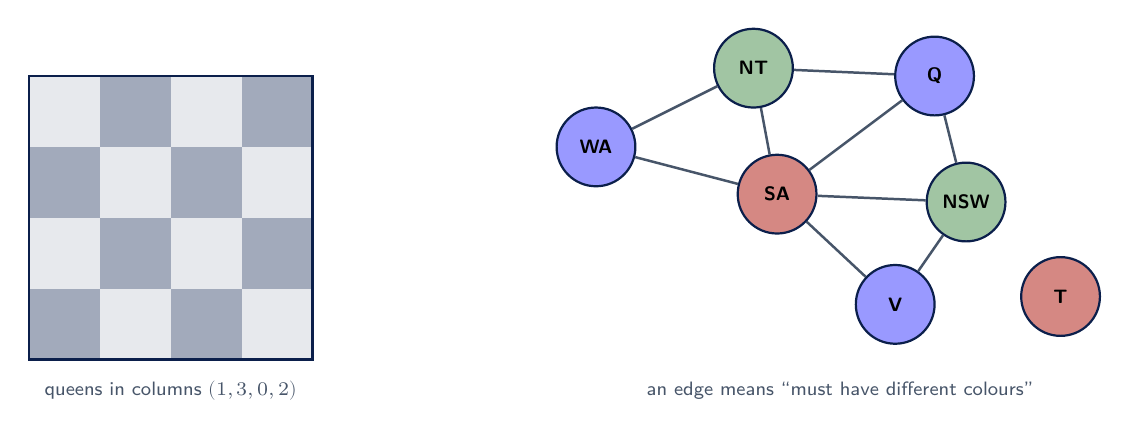
\begin{tikzpicture}[x=1cm,y=1cm]
  \foreach \r in {0,1,2,3} \foreach \c in {0,1,2,3}{
    \pgfmathtruncatemacro{\k}{mod(\r+\c,2)}
    \ifnum\k=0 \fill[navy!10] (\c*0.9,-\r*0.9) rectangle ++(0.9,-0.9); \else \fill[navy!38] (\c*0.9,-\r*0.9) rectangle ++(0.9,-0.9); \fi}
  \draw[navy,line width=1pt] (0,0) rectangle (3.6,-3.6);
  \foreach \r/\c in {0/1,1/3,2/0,3/2} \node[text=crimson,font=\LARGE] at (\c*0.9+0.45,-\r*0.9-0.45) {\queen};
  \node[lbl] at (1.8,-4.0) {queens in columns $(1,3,0,2)$};
  \begin{scope}[shift={(7.2,-0.9)},every node/.style={circle,draw=navy,line width=0.8pt,minimum size=10mm,font=\sffamily\bfseries\scriptsize,inner sep=0pt}]
    \node[fill=blue!40] (WA) at (0,0) {WA};
    \node[fill=dgreen!45] (NT) at (2.0,1.0) {NT};
    \node[fill=crimson!55] (SA) at (2.3,-0.6) {SA};
    \node[fill=blue!40] (Q) at (4.3,0.9) {Q};
    \node[fill=dgreen!45] (NSW) at (4.7,-0.7) {NSW};
    \node[fill=blue!40] (V) at (3.8,-2.0) {V};
    \node[fill=crimson!55] (T) at (5.9,-1.9) {T};
    \foreach \a/\b in {WA/NT,WA/SA,NT/SA,NT/Q,SA/Q,SA/NSW,SA/V,Q/NSW,NSW/V} \draw[slate,line width=0.9pt] (\a)--(\b);
  \end{scope}
  \node[lbl] at (10.3,-4.0) {an edge means ``must have different colours''};
\end{tikzpicture}
\end{diagram}

\begin{example}
\textbf{4-Queens trace} (one queen per row, columns numbered 0 to 3):
\begin{itemize}
  \item Row 0 $\to$ column 0. Row 1: columns 0, 1 attacked, place at 2. Row 2: every column attacked $\Rightarrow$ \textbf{backtrack}.
  \item Row 1 $\to$ column 3. Row 2 $\to$ column 1. Row 3: every column attacked $\Rightarrow$ \textbf{backtrack} up to row 0.
  \item Row 0 $\to$ column 1. Row 1 $\to$ 3. Row 2 $\to$ 0. Row 3 $\to$ 2. \textbf{Solution} $(1,3,0,2)$.
\end{itemize}
\end{example}

\begin{maths}
A CSP is a triple $\langle X, D, C\rangle$: variables $X=\{X_1,\dots,X_n\}$, domains $D_i$, and constraints $C$.

\textbf{N-Queens.} $X_i$ = column of the queen in row $i$, $D_i=\{0,\dots,N-1\}$, and for all $i<j$:
\[ X_i \ne X_j \qquad\text{and}\qquad |X_i - X_j| \ne j-i . \]
Complete assignments number $N^{N}$ ($8^{8}=16{,}777{,}216$), permutations $N!$ ($8! = 40{,}320$), yet only 92 are solutions for $N=8$. Backtracking visits a tiny fraction of this space.

\textbf{Map colouring.} For the constraint graph $G=(V,E)$ find $c: V\to\{R,G,B\}$ with
\[ c(u)\ne c(v)\quad \text{for every edge } (u,v)\in E . \]
The smallest number of colours that works is the chromatic number $\chi(G)$; for Australia $\chi=3$ because SA, NT and Q are mutually adjacent.

\textbf{Degree heuristic:} choose next the variable involved in the largest number of constraints (here SA with 5 neighbours), which reduces later failures. Worst-case time of backtracking is $O(d^{n})$ for domain size $d$.
\end{maths}

\begin{algorithm}
\begin{enumerate}
  \item If every variable is assigned, return the assignment as a solution.
  \item Select an unassigned variable.
  \item For each value in its domain: if the value is consistent with the current assignment, assign it and recurse.
  \item If the recursive call succeeds, return the solution; otherwise remove the assignment (backtrack) and try the next value.
  \item If no value works, return failure to the caller.
\end{enumerate}
\end{algorithm}

\begin{pycode}{exp05\_csp\_backtracking.py}
"""Experiment 5: Constraint Satisfaction by Backtracking.
Part A: N-Queens.   Part B: Map colouring of Australia."""


# ---------------- Part A: N-Queens ----------------
def safe(queens, row, col):
    """queens[r] = column of the queen already placed in row r."""
    for r, c in enumerate(queens):
        if c == col or abs(c - col) == row - r:
            return False
    return True


def n_queens(n):
    """Return (first solution, number of solutions, number of backtracks)."""
    solutions, stats = [], {"backtracks": 0}

    def place(queens):
        row = len(queens)
        if row == n:
            solutions.append(tuple(queens))
            return
        for col in range(n):
            if safe(queens, row, col):
                queens.append(col)
                place(queens)
                queens.pop()                 # undo the choice: BACKTRACK
                stats["backtracks"] += 1

    place([])
    first = solutions[0] if solutions else None
    return first, len(solutions), stats["backtracks"]


def show_board(solution):
    n = len(solution)
    for r in range(n):
        print("   " + " ".join("Q" if solution[r] == c else "." for c in range(n)))


# ---------------- Part B: Map colouring ----------------
NEIGHBOURS = {
    "WA": ["NT", "SA"],
    "NT": ["WA", "SA", "Q"],
    "SA": ["WA", "NT", "Q", "NSW", "V"],
    "Q": ["NT", "SA", "NSW"],
    "NSW": ["Q", "SA", "V"],
    "V": ["SA", "NSW"],
    "T": [],
}
COLOURS = ["Red", "Green", "Blue"]


def consistent(region, colour, assignment):
    return all(assignment.get(nb) != colour for nb in NEIGHBOURS[region])


def select_unassigned(assignment):
    """Degree heuristic: pick the unassigned region with most neighbours."""
    free = [r for r in NEIGHBOURS if r not in assignment]
    return max(free, key=lambda r: len(NEIGHBOURS[r]))


def colour_map(assignment, trace):
    if len(assignment) == len(NEIGHBOURS):
        return assignment
    region = select_unassigned(assignment)
    for colour in COLOURS:
        if consistent(region, colour, assignment):
            assignment[region] = colour
            trace.append(f"assign {region:<3} = {colour}")
            result = colour_map(assignment, trace)
            if result:
                return result
            del assignment[region]           # BACKTRACK
            trace.append(f"undo   {region}")
    return None


if __name__ == "__main__":
    print("PART A: N-Queens by backtracking")
    print("   N  solutions  backtracks")
    for n in range(4, 9):
        _, count, back = n_queens(n)
        print(f"  {n:2d}  {count:9d}  {back:10d}")
    first, _, _ = n_queens(8)
    print("First solution for N = 8 (column of queen in each row):", first)
    show_board(first)

    print("\nPART B: Map colouring of Australia with 3 colours")
    trace = []
    result = colour_map({}, trace)
    for line in trace:
        print("  ", line)
    print("Final assignment:")
    for region in NEIGHBOURS:
        print(f"   {region:<3} -> {result[region]}")
    ok = all(result[r] != result[nb] for r in NEIGHBOURS for nb in NEIGHBOURS[r])
    print("All constraints satisfied:", ok)
\end{pycode}

\begin{inputbox}
Part A: board sizes $N = 4$ to $8$. Part B: the adjacency list \texttt{NEIGHBOURS} of the seven Australian states and territories and the colour list \texttt{["Red", "Green", "Blue"]}. Try removing \texttt{"Blue"}: the program then reports that no colouring exists.
\end{inputbox}

\begin{outputbox}
PART A: N-Queens by backtracking
   N  solutions  backtracks
   4          2          16
   5         10          53
   6          4         152
   7         40         551
   8         92        2056
First solution for N = 8 (column of queen in each row): (0, 4, 7, 5, 2, 6, 1, 3)
   Q . . . . . . .
   . . . . Q . . .
   . . . . . . . Q
   . . . . . Q . .
   . . Q . . . . .
   . . . . . . Q .
   . Q . . . . . .
   . . . Q . . . .

PART B: Map colouring of Australia with 3 colours
   assign SA  = Red
   assign NT  = Green
   assign Q   = Blue
   assign NSW = Green
   assign WA  = Blue
   assign V   = Blue
   assign T   = Red
Final assignment:
   WA  -> Blue
   NT  -> Green
   SA  -> Red
   Q   -> Blue
   NSW -> Green
   V   -> Blue
   T   -> Red
All constraints satisfied: True
\end{outputbox}

\begin{result}
Backtracking found all solutions of N-Queens for $N=4$ to $8$ (92 solutions for $N=8$) and a valid 3-colouring of the map of Australia without any backtracking step, thanks to the degree heuristic.
\end{result}

\begin{viva}
\begin{enumerate}
  \item Define variables, domains and constraints for Sudoku.
  \item How is backtracking different from generate-and-test?
  \item What are the MRV and least-constraining-value heuristics?
  \item What is forward checking? What is arc consistency (AC-3)?
  \item Why can Tasmania be given any colour in the map-colouring problem?
\end{enumerate}
\end{viva}
% ============================ EXPERIMENT 6 ===========================
\experiment{Representing Facts and Rules and Answering Queries by Logical Inference (Prolog / Python)}{CO204.3}{Facts, Rules and Inference}

\begin{aim}
To represent knowledge as facts and rules (Horn clauses) and to answer queries by logical inference, using a Prolog-style forward-chaining engine written in Python.
\end{aim}

\begin{descr}
A \textbf{knowledge base} (KB) stores what is known; an \textbf{inference engine} derives what follows.
\begin{itemize}
  \item A \textbf{fact} is an unconditional statement: \texttt{parent(ram, lav)}.
  \item A \textbf{rule} is a conditional statement: \texttt{grandparent(X, Z) :- parent(X, Y), parent(Y, Z)}.
  \item A \textbf{query} asks whether something follows from the KB, or for which values of the variables it follows.
\end{itemize}
As in Prolog, names starting with a capital letter are variables. The Python engine applies every rule to the known facts again and again (forward chaining) until nothing new is produced; queries are then answered by pattern matching.
\end{descr}

\begin{diagram}{family tree used as the knowledge base, and the inference pipeline}
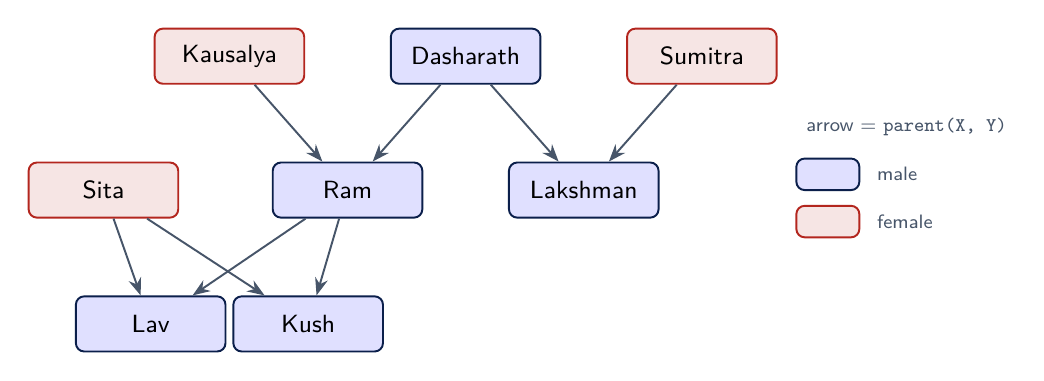
\begin{tikzpicture}[x=1cm,y=1cm,
  ml/.style={st,fill=blue!12,minimum width=19mm},fm/.style={st,fill=crimson!12,draw=crimson,minimum width=19mm}]
  \node[fm] (ka) at (-3,0) {Kausalya}; \node[ml] (da) at (0,0) {Dasharath}; \node[fm] (su) at (3,0) {Sumitra};
  \node[fm] (si) at (-4.6,-1.7) {Sita}; \node[ml] (ra) at (-1.5,-1.7) {Ram}; \node[ml] (la) at (1.5,-1.7) {Lakshman};
  \node[ml] (lv) at (-4.0,-3.4) {Lav}; \node[ml] (ku) at (-2.0,-3.4) {Kush};
  \foreach \p/\c in {ka/ra,da/ra,da/la,su/la,si/lv,si/ku,ra/lv,ra/ku} \draw[arr] (\p) -- (\c);
  \node[lbl] at (5.6,-0.9) {arrow = \texttt{parent(X, Y)}};
  \node[ml,minimum width=8mm,minimum height=4mm] at (4.6,-1.5) {}; \node[lbl,anchor=west] at (5.1,-1.5) {male};
  \node[fm,minimum width=8mm,minimum height=4mm] at (4.6,-2.1) {}; \node[lbl,anchor=west] at (5.1,-2.1) {female};
\end{tikzpicture}

\vspace{5pt}
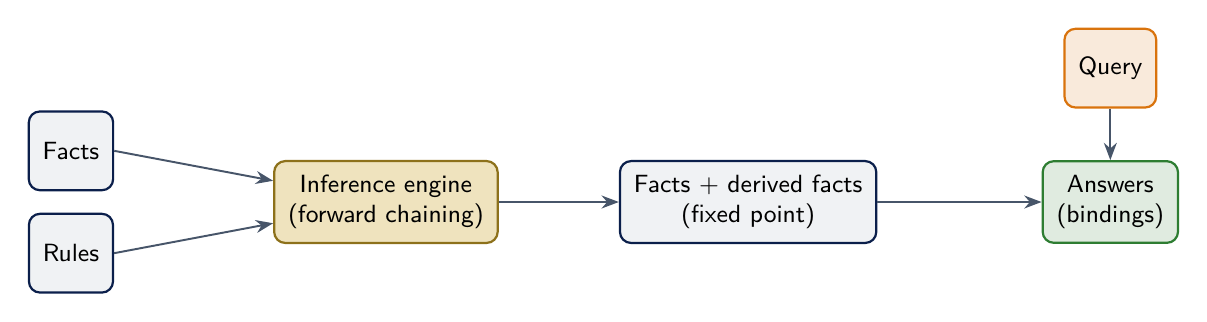
\begin{tikzpicture}[x=1cm,y=1cm]
  \node[blk] (f) at (0,0.65) {Facts}; \node[blk] (r) at (0,-0.65) {Rules};
  \node[blk,fill=gold!30,draw=gold!70!black] (e) at (4.0,0) {Inference engine\\ (forward chaining)};
  \node[blk] (d) at (8.6,0) {Facts + derived facts\\ (fixed point)};
  \node[blk,fill=dgreen!15,draw=dgreen] (a) at (13.2,0) {Answers\\ (bindings)};
  \node[blk,fill=orange!15,draw=orange] (q) at (13.2,1.7) {Query};
  \draw[arr] (f.east) -- (e); \draw[arr] (r.east) -- (e); \draw[arr] (e) -- (d); \draw[arr] (d) -- (a); \draw[arr] (q) -- (a);
\end{tikzpicture}
\end{diagram}

\begin{example}
Query: \texttt{?- grandparent(X, kush).}\quad Using the rule with $Z=\texttt{kush}$:
\begin{itemize}
  \item \texttt{parent(Y, kush)} matches with $Y=\texttt{ram}$ and $Y=\texttt{sita}$.
  \item \texttt{parent(X, ram)} matches with $X=\texttt{dasharath}$ and $X=\texttt{kausalya}$; \texttt{parent(X, sita)} matches nothing.
\end{itemize}
Answer: $X=\texttt{dasharath}$; $X=\texttt{kausalya}$.
\end{example}

\begin{plaincode}{THE SAME KNOWLEDGE BASE IN PROLOG (for SWI-Prolog)}
parent(dasharath, ram).   parent(kausalya, ram).
parent(dasharath, lakshman).   parent(sumitra, lakshman).
parent(ram, lav).  parent(sita, lav).  parent(ram, kush).  parent(sita, kush).
male(dasharath). male(ram). male(lakshman). male(lav). male(kush).
female(kausalya). female(sumitra). female(sita).

father(X, Y)      :- parent(X, Y), male(X).
mother(X, Y)      :- parent(X, Y), female(X).
grandparent(X, Z) :- parent(X, Y), parent(Y, Z).
sibling(X, Y)     :- parent(P, X), parent(P, Y), X \= Y.
ancestor(X, Y)    :- parent(X, Y).
ancestor(X, Z)    :- parent(X, Y), ancestor(Y, Z).

?- grandparent(X, kush).
\end{plaincode}

\begin{maths}
\textbf{Horn clause:} a disjunction of literals with at most one positive literal. A rule
\[ B_1 \land B_2 \land \dots \land B_k \Rightarrow H \quad\equiv\quad \lnot B_1 \lor \dots \lor \lnot B_k \lor H \]
is a definite clause; a fact is a definite clause with $k=0$.

\textbf{Rules of this experiment in first-order logic:}
\begin{align*}
&\forall x\,\forall y\;\; \mathit{Parent}(x,y)\land \mathit{Male}(x) \Rightarrow \mathit{Father}(x,y)\\
&\forall x\,\forall y\,\forall z\;\; \mathit{Parent}(x,y)\land \mathit{Parent}(y,z) \Rightarrow \mathit{Grandparent}(x,z)\\
&\forall x\,\forall y\,\forall z\;\; \mathit{Parent}(x,y)\land \mathit{Ancestor}(y,z) \Rightarrow \mathit{Ancestor}(x,z)
\end{align*}
\textbf{Generalised Modus Ponens:} if $\theta$ is a substitution with $p_i'\theta = p_i\theta$ for all $i$, then
\[ \frac{p_1',\; p_2',\;\dots,\; p_k',\qquad (p_1\land p_2\land\dots\land p_k \Rightarrow q)}{q\,\theta} \]
\textbf{Forward chaining as a fixed point:} let $T(F)= F \cup \{\,q\theta \mid \text{a rule fires on facts in } F\,\}$. Starting from the base facts $F_0$, compute $F_{i+1}=T(F_i)$ until $F_{i+1}=F_i$. For a KB without function symbols this always terminates, and the result contains exactly the atomic facts entailed by the KB (sound and complete for definite clauses).
\end{maths}

\begin{algorithm}
\begin{enumerate}
  \item Store the base facts in a set.
  \item For every rule, find all variable bindings that make every body literal match a known fact.
  \item For each binding, instantiate the head; if it is a new fact, add it.
  \item Repeat steps 2 and 3 until a complete round adds no new fact (fixed point).
  \item To answer a query, match it against the final fact set and report the bindings (or true / false).
\end{enumerate}
\end{algorithm}

\begin{pycode}{exp06\_facts\_rules\_inference.py}
"""Experiment 6: Facts, rules and logical inference (Prolog style) in Python.
Convention (same as Prolog): names starting with an UPPER-case letter are
variables, lower-case names are constants."""

FACTS = {
    ("male", "dasharath"), ("male", "ram"), ("male", "lakshman"),
    ("male", "lav"), ("male", "kush"),
    ("female", "kausalya"), ("female", "sumitra"), ("female", "sita"),
    ("parent", "dasharath", "ram"), ("parent", "kausalya", "ram"),
    ("parent", "dasharath", "lakshman"), ("parent", "sumitra", "lakshman"),
    ("parent", "ram", "lav"), ("parent", "sita", "lav"),
    ("parent", "ram", "kush"), ("parent", "sita", "kush"),
}

# Each rule is (head, [body literals]) and reads:  head :- body1, body2, ...
RULES = [
    (("father", "X", "Y"), [("parent", "X", "Y"), ("male", "X")]),
    (("mother", "X", "Y"), [("parent", "X", "Y"), ("female", "X")]),
    (("grandparent", "X", "Z"), [("parent", "X", "Y"), ("parent", "Y", "Z")]),
    (("sibling", "X", "Y"), [("parent", "P", "X"), ("parent", "P", "Y"),
                             ("neq", "X", "Y")]),
    (("ancestor", "X", "Y"), [("parent", "X", "Y")]),
    (("ancestor", "X", "Z"), [("parent", "X", "Y"), ("ancestor", "Y", "Z")]),
]


def is_var(term):
    return term[0].isupper()


def match(pattern, fact, env):
    """Try to match a literal against a ground fact; extend bindings."""
    if pattern[0] != fact[0] or len(pattern) != len(fact):
        return None
    env = dict(env)
    for p, f in zip(pattern[1:], fact[1:]):
        if is_var(p):
            if env.setdefault(p, f) != f:
                return None
        elif p != f:
            return None
    return env


def solve(body, facts, env):
    """Yield every binding that satisfies all literals of the body."""
    if not body:
        yield env
        return
    first, rest = body[0], body[1:]
    if first[0] == "neq":                       # built-in: X \= Y
        a, b = (env.get(t, t) for t in first[1:])
        if a != b:
            yield from solve(rest, facts, env)
        return
    for fact in facts:
        new_env = match(first, fact, env)
        if new_env is not None:
            yield from solve(rest, facts, new_env)


def forward_chain(facts, rules):
    """Apply Modus Ponens repeatedly until no new fact can be derived."""
    facts, rounds = set(facts), 0
    while True:
        new = set()
        for head, body in rules:
            for env in solve(body, facts, {}):
                derived = tuple(env.get(t, t) for t in head)
                if derived not in facts:
                    new.add(derived)
        if not new:
            return facts, rounds
        facts |= new
        rounds += 1
        print(f"   round {rounds}: {len(new)} new facts derived")


def ask(query, kb):
    """Answer a query; variables in the query are reported as bindings."""
    answers = sorted({tuple(sorted(env.items()))
                      for env in solve([query], kb, {})})
    text = f"?- {query[0]}({', '.join(query[1:])})."
    if not any(is_var(t) for t in query[1:]):
        print(f"{text:<34} {'true' if answers else 'false'}")
    elif not answers:
        print(f"{text:<34} false")
    else:
        shown = "; ".join(", ".join(f"{v} = {c}" for v, c in a) for a in answers)
        print(f"{text:<34} {shown}")


if __name__ == "__main__":
    print(f"Base facts: {len(FACTS)}, rules: {len(RULES)}")
    kb, rounds = forward_chain(FACTS, RULES)
    print(f"Fixed point after {rounds} rounds: {len(kb)} facts in total\n")
    for q in [("father", "dasharath", "ram"),
              ("mother", "sita", "ram"),
              ("father", "X", "lav"),
              ("grandparent", "X", "kush"),
              ("sibling", "lav", "Y"),
              ("ancestor", "dasharath", "D"),
              ("sibling", "ram", "S")]:
        ask(q, kb)
\end{pycode}

\begin{inputbox}
16 base facts (\texttt{male}, \texttt{female}, \texttt{parent}), 6 rules, and 7 queries listed at the bottom of the program. Add your own facts, for example \texttt{("parent", "lakshman", "angad")}, and ask \texttt{("ancestor", "X", "angad")}.
\end{inputbox}

\begin{outputbox}
Base facts: 16, rules: 6
   round 1: 24 new facts derived
   round 2: 4 new facts derived
Fixed point after 2 rounds: 44 facts in total

?- father(dasharath, ram).         true
?- mother(sita, ram).              false
?- father(X, lav).                 X = ram
?- grandparent(X, kush).           X = dasharath; X = kausalya
?- sibling(lav, Y).                Y = kush
?- ancestor(dasharath, D).         D = kush; D = lakshman; D = lav; D = ram
?- sibling(ram, S).                S = lakshman
\end{outputbox}

\begin{result}
Facts and rules were represented as Horn clauses. Forward chaining derived 28 new facts in two rounds, and the queries were answered correctly, including the recursive \texttt{ancestor} relation.
\end{result}

\begin{viva}
\begin{enumerate}
  \item Differentiate between a fact, a rule and a query in Prolog.
  \item What is the difference between forward chaining and backward chaining? Which one does Prolog use?
  \item What is a Horn clause? Why are Horn clauses convenient for inference?
  \item What is the closed-world assumption (negation as failure)?
  \item Why is the test \texttt{X \textbackslash= Y} needed in the \texttt{sibling} rule?
\end{enumerate}
\end{viva}

% ============================ EXPERIMENT 7 ===========================
\experiment{Unification and Resolution for First-Order Logic Statements}{CO204.3}{Unification and Resolution}

\begin{aim}
To implement the unification algorithm (with occurs check) and to prove a first-order logic statement by resolution refutation.
\end{aim}

\begin{descr}
\textbf{Unification} finds a substitution $\theta$ that makes two logical expressions identical, e.g. \textit{Knows(John, x)} and \textit{Knows(y, Bill)} become identical under $\theta=\{y/\mathit{John},\,x/\mathit{Bill}\}$. The most general such substitution is the \emph{most general unifier} (MGU).

\textbf{Resolution} is a single inference rule that is complete for first-order logic when used for \emph{refutation}: to prove $\alpha$ from KB, convert KB and $\lnot\alpha$ into clauses (CNF) and resolve pairs of clauses containing complementary literals until the \emph{empty clause} appears. The empty clause signals a contradiction, so KB entails $\alpha$.
\end{descr}

\begin{diagram}{resolution refutation proving Evil(John)}
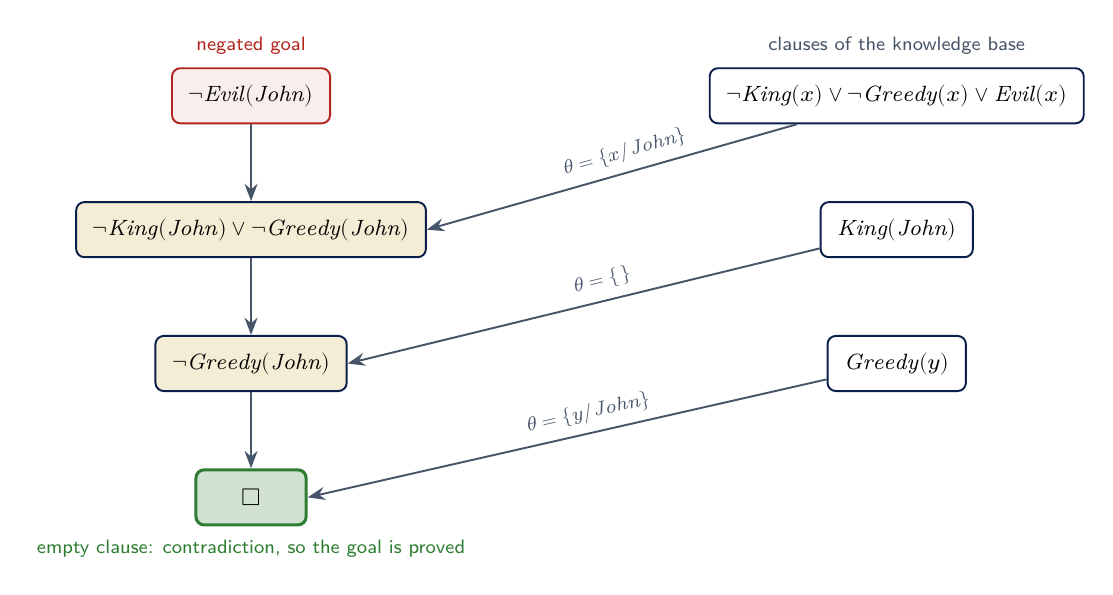
\begin{tikzpicture}[x=1cm,y=1cm,cl/.style={st,font=\sffamily\footnotesize,inner xsep=6pt}]
  \node[cl,draw=crimson,fill=crimson!8] (g0) at (0,0) {$\lnot \mathit{Evil}(\mathit{John})$};
  \node[cl] (c1) at (8.2,0) {$\lnot \mathit{King}(x)\lor\lnot \mathit{Greedy}(x)\lor \mathit{Evil}(x)$};
  \node[cl,fill=gold!20] (g1) at (0,-1.7) {$\lnot \mathit{King}(\mathit{John})\lor\lnot \mathit{Greedy}(\mathit{John})$};
  \node[cl] (c2) at (8.2,-1.7) {$\mathit{King}(\mathit{John})$};
  \node[cl,fill=gold!20] (g2) at (0,-3.4) {$\lnot \mathit{Greedy}(\mathit{John})$};
  \node[cl] (c3) at (8.2,-3.4) {$\mathit{Greedy}(y)$};
  \node[goal,minimum width=14mm] (g3) at (0,-5.1) {$\square$};
  \draw[arr] (g0) -- (g1); \draw[arr] (c1) -- node[lbl,sloped,above,pos=0.45]{$\theta=\{x/\mathit{John}\}$} (g1.east);
  \draw[arr] (g1) -- (g2); \draw[arr] (c2) -- node[lbl,sloped,above,pos=0.45]{$\theta=\{\,\}$} (g2.east);
  \draw[arr] (g2) -- (g3); \draw[arr] (c3) -- node[lbl,sloped,above,pos=0.45]{$\theta=\{y/\mathit{John}\}$} (g3.east);
  \node[lbl,text=crimson,above] at (0,0.4) {negated goal};
  \node[lbl,above] at (8.2,0.4) {clauses of the knowledge base};
  \node[lbl,text=dgreen] at (0,-5.75) {empty clause: contradiction, so the goal is proved};
\end{tikzpicture}
\end{diagram}

\begin{example}
Unify $\mathit{Knows}(\mathit{John}, x)$ with $\mathit{Knows}(y, \mathit{Mother}(y))$:
\begin{enumerate}
  \item Predicate symbols and arity agree (\textit{Knows}/2).
  \item First arguments: \textit{John} and $y$ $\Rightarrow$ $\theta=\{y/\mathit{John}\}$.
  \item Second arguments: $x$ and $\mathit{Mother}(y)$. Under $\theta$ the second term is $\mathit{Mother}(\mathit{John})$, so bind $x$ to it.
  \item Result: $\theta=\{y/\mathit{John},\ x/\mathit{Mother}(\mathit{John})\}$.
\end{enumerate}
$\mathit{P}(x)$ and $\mathit{P}(f(x))$ do \emph{not} unify: $x$ occurs inside $f(x)$ (occurs check).
\end{example}

\begin{maths}
\textbf{Substitution and unifier:} $\theta=\{v_1/t_1,\dots,v_n/t_n\}$ replaces variable $v_i$ by term $t_i$. $\theta$ unifies $p$ and $q$ if $p\theta = q\theta$. $\theta$ is an MGU if every other unifier $\sigma$ can be written as $\sigma=\theta\lambda$ for some substitution $\lambda$.

\textbf{Binary resolution rule:} if $\theta=\mathrm{MGU}(\ell_i,\ m_j)$ for a positive literal $\ell_i$ and a negated literal $\lnot m_j$, then
\[ \frac{\ell_1\lor\dots\lor \ell_i \lor\dots\lor \ell_k,\qquad m_1\lor\dots\lor \lnot m_j\lor\dots\lor m_n}
{(\ell_1\lor\dots\lor \ell_{i-1}\lor \ell_{i+1}\lor\dots\lor \ell_k\lor m_1\lor\dots\lor m_{j-1}\lor m_{j+1}\lor\dots\lor m_n)\,\theta} \]
\textbf{Refutation principle:}\quad $KB \models \alpha \iff KB\land\lnot\alpha$ is unsatisfiable $\iff$ the empty clause $\square$ can be derived.

\textbf{Conversion to CNF:} (1) eliminate $\Rightarrow$ and $\Leftrightarrow$; (2) move $\lnot$ inwards; (3) standardise variables apart; (4) Skolemise existential quantifiers; (5) drop universal quantifiers; (6) distribute $\lor$ over $\land$.

\textbf{Example of step (1):}\quad $\mathit{Missile}(x)\Rightarrow \mathit{Weapon}(x)$ becomes $\lnot \mathit{Missile}(x)\lor \mathit{Weapon}(x)$.
\end{maths}

\begin{algorithm}
\textbf{Unify($x$, $y$, $\theta$)}
\begin{enumerate}
  \item Apply $\theta$ to $x$ and $y$. If they are identical, return $\theta$.
  \item If $x$ is a variable: fail if $x$ occurs in $y$, otherwise return $\theta\cup\{x/y\}$. Treat a variable $y$ symmetrically.
  \item If both are compound with the same functor and arity, unify the arguments from left to right, passing $\theta$ along.
  \item Otherwise fail.
\end{enumerate}
\textbf{Resolution refutation}
\begin{enumerate}
  \item Write the KB in clause form and add the negated goal as the current clause.
  \item Pick the first literal of the current clause and find a KB clause (with renamed variables) containing a complementary literal that unifies with it.
  \item Form the resolvent, apply $\theta$, and make it the current clause.
  \item If the current clause is empty, the goal is proved; if no clause can be resolved, backtrack.
\end{enumerate}
\end{algorithm}

\begin{pycode}{exp07\_unification\_resolution.py}
"""Experiment 7: Unification and Resolution for First-Order Logic.
Terms : variable  -> string starting with '?'      e.g. '?x'
        constant  -> any other string              e.g. 'John'
        compound  -> tuple (functor, arg1, ...)    e.g. ('Knows', 'John', '?x')
Literal: (sign, atom) where sign is True for positive, False for negated."""


def is_var(t):
    return isinstance(t, str) and t.startswith("?")


def substitute(t, theta):
    """Apply substitution theta to term t."""
    if is_var(t):
        return substitute(theta[t], theta) if t in theta else t
    if isinstance(t, tuple):
        return tuple(substitute(a, theta) for a in t)
    return t


def occurs(var, t, theta):
    """Occurs check: does var appear inside t?  (blocks x = f(x))"""
    t = substitute(t, theta)
    if var == t:
        return True
    return isinstance(t, tuple) and any(occurs(var, a, theta) for a in t)


def unify(x, y, theta=None):
    """Return the most general unifier of x and y, or None on failure."""
    theta = {} if theta is None else theta
    x, y = substitute(x, theta), substitute(y, theta)
    if x == y:
        return theta
    if is_var(x):
        return None if occurs(x, y, theta) else {**theta, x: y}
    if is_var(y):
        return unify(y, x, theta)
    if isinstance(x, tuple) and isinstance(y, tuple) and len(x) == len(y):
        for a, b in zip(x, y):
            theta = unify(a, b, theta)
            if theta is None:
                return None
        return theta
    return None


def show(t):
    if isinstance(t, tuple):
        return f"{t[0]}({', '.join(show(a) for a in t[1:])})"
    return t.lstrip("?")


def show_theta(theta):
    if theta is None:
        return "FAIL"
    return "{" + ", ".join(f"{show(v)}/{show(substitute(v, theta))}"
                           for v in theta) + "}"


def show_clause(clause):
    if not clause:
        return "[] (empty clause)"
    return " v ".join(("" if sign else "~") + show(atom) for sign, atom in clause)


def rename(clause, n):
    """Standardise variables apart by attaching a unique suffix."""
    def r(t):
        if is_var(t):
            return f"{t}{n}"
        return tuple(r(a) for a in t) if isinstance(t, tuple) else t
    return [(sign, r(atom)) for sign, atom in clause]


def refute(kb, goal, limit=15):
    """Linear resolution refutation: repeatedly resolve the first literal
    of the current goal clause with a complementary literal of a KB clause."""
    counter = [0]

    def solve(goal, depth, proof):
        if not goal:
            return proof                          # empty clause derived
        if depth == 0:
            return None
        sign, atom = goal[0]
        for idx, clause in enumerate(kb, 1):
            counter[0] += 1
            clause = rename(clause, counter[0])
            for k, (sign2, atom2) in enumerate(clause):
                if sign2 == sign:
                    continue                      # need opposite signs
                theta = unify(atom, atom2)
                if theta is None:
                    continue
                rest = goal[1:] + clause[:k] + clause[k + 1:]
                resolvent = []
                for s, a in rest:
                    lit = (s, substitute(a, theta))
                    if lit not in resolvent:
                        resolvent.append(lit)
                found = solve(resolvent, depth - 1,
                              proof + [(idx, theta, resolvent)])
                if found is not None:
                    return found
        return None

    return solve(goal, limit, [])


if __name__ == "__main__":
    print("PART A: Unification")
    pairs = [
        (("Knows", "John", "?x"), ("Knows", "John", "Jane")),
        (("Knows", "John", "?x"), ("Knows", "?y", "Bill")),
        (("Knows", "John", "?x"), ("Knows", "?y", ("Mother", "?y"))),
        (("P", "?x", ("f", "?y")), ("P", ("g", "?z"), ("f", "A"))),
        (("Knows", "John", "?x"), ("Knows", "?x", "Elizabeth")),
        (("P", "?x"), ("P", ("f", "?x"))),
    ]
    for a, b in pairs:
        print(f"   {show(a):<18} , {show(b):<22} => {show_theta(unify(a, b))}")

    print("\nPART B: Resolution refutation (Colonel West is a criminal)")
    kb = [
        [(False, ("American", "?x")), (False, ("Weapon", "?y")),
         (False, ("Sells", "?x", "?y", "?z")), (False, ("Hostile", "?z")),
         (True, ("Criminal", "?x"))],
        [(False, ("Missile", "?x")), (False, ("Owns", "Nono", "?x")),
         (True, ("Sells", "West", "?x", "Nono"))],
        [(False, ("Missile", "?x")), (True, ("Weapon", "?x"))],
        [(False, ("Enemy", "?x", "America")), (True, ("Hostile", "?x"))],
        [(True, ("Owns", "Nono", "M1"))],
        [(True, ("Missile", "M1"))],
        [(True, ("American", "West"))],
        [(True, ("Enemy", "Nono", "America"))],
    ]
    for i, clause in enumerate(kb, 1):
        print(f"   C{i}: {show_clause(clause)}")
    goal = [(False, ("Criminal", "West"))]
    print(f"   Negated goal G0: {show_clause(goal)}")
    proof = refute(kb, goal)
    for step, (idx, theta, resolvent) in enumerate(proof, 1):
        print(f"   G{step}: resolve G{step - 1} with C{idx} "
              f"=> {show_clause(resolvent)}")
    print("   Empty clause reached: KB entails Criminal(West).")
\end{pycode}

\begin{inputbox}
Part A: six pairs of expressions (variables are written with a leading \texttt{?} in the code). Part B: the ``Colonel West'' knowledge base in clause form (C1 to C8) and the goal \textit{Criminal(West)}, entered in negated form. In the output \texttt{\textasciitilde} means NOT, \texttt{v} means OR, and names such as \texttt{y1} or \texttt{x11} are variables renamed during standardising apart.
\end{inputbox}

\begin{outputbox}
PART A: Unification
   Knows(John, x)     , Knows(John, Jane)      => {x/Jane}
   Knows(John, x)     , Knows(y, Bill)         => {y/John, x/Bill}
   Knows(John, x)     , Knows(y, Mother(y))    => {y/John, x/Mother(John)}
   P(x, f(y))         , P(g(z), f(A))          => {x/g(z), y/A}
   Knows(John, x)     , Knows(x, Elizabeth)    => FAIL
   P(x)               , P(f(x))                => FAIL

PART B: Resolution refutation (Colonel West is a criminal)
   C1: ~American(x) v ~Weapon(y) v ~Sells(x, y, z) v ~Hostile(z) v Criminal(x)
   C2: ~Missile(x) v ~Owns(Nono, x) v Sells(West, x, Nono)
   C3: ~Missile(x) v Weapon(x)
   C4: ~Enemy(x, America) v Hostile(x)
   C5: Owns(Nono, M1)
   C6: Missile(M1)
   C7: American(West)
   C8: Enemy(Nono, America)
   Negated goal G0: ~Criminal(West)
   G1: resolve G0 with C1 => ~American(West) v ~Weapon(y1) v ~Sells(West, y1, z1) v ~Hostile(z1)
   G2: resolve G1 with C7 => ~Weapon(y1) v ~Sells(West, y1, z1) v ~Hostile(z1)
   G3: resolve G2 with C3 => ~Sells(West, x11, z1) v ~Hostile(z1) v ~Missile(x11)
   G4: resolve G3 with C2 => ~Hostile(Nono) v ~Missile(x13) v ~Owns(Nono, x13)
   G5: resolve G4 with C4 => ~Missile(x13) v ~Owns(Nono, x13) v ~Enemy(Nono, America)
   G6: resolve G5 with C6 => ~Owns(Nono, M1) v ~Enemy(Nono, America)
   G7: resolve G6 with C5 => ~Enemy(Nono, America)
   G8: resolve G7 with C8 => [] (empty clause)
   Empty clause reached: KB entails Criminal(West).
\end{outputbox}

\begin{result}
The unification algorithm produced the most general unifiers and correctly rejected the two non-unifiable pairs. Resolution refutation derived the empty clause in 8 steps, proving that Colonel West is a criminal.
\end{result}

\begin{viva}
\begin{enumerate}
  \item What is a most general unifier? Give an example of a unifier that is not most general.
  \item Why is the occurs check necessary?
  \item What is Skolemisation and when is it required?
  \item Why is resolution used with refutation and not for direct proof?
  \item What does ``standardising variables apart'' mean and why is it done?
\end{enumerate}
\end{viva}

% ============================ EXPERIMENT 8 ===========================
\experiment{Bayes' Theorem and a Simple Bayesian Network for a Diagnostic Reasoning Problem}{CO204.4}{Bayes and Bayesian Networks}

\begin{aim}
To apply Bayes' theorem to a medical-test diagnosis problem and to perform exact inference by enumeration on the burglary-alarm Bayesian network.
\end{aim}

\begin{descr}
Real-world knowledge is uncertain. \textbf{Bayes' theorem} turns \emph{causal} knowledge, $P(\text{evidence}\mid\text{cause})$, into the \emph{diagnostic} belief we actually need, $P(\text{cause}\mid\text{evidence})$. A \textbf{Bayesian network} is a directed acyclic graph whose nodes are random variables; each node stores a conditional probability table (CPT) given its parents. The network represents the full joint distribution compactly, and any query can be answered by summing the joint over the hidden variables.

\textbf{Scenario.} A burglar alarm can be triggered by a burglary or by an earthquake. Neighbours John and Mary promise to call when they hear the alarm. Both have called: how likely is a burglary?
\end{descr}

\begin{diagram}{the burglary-alarm Bayesian network with its CPTs}
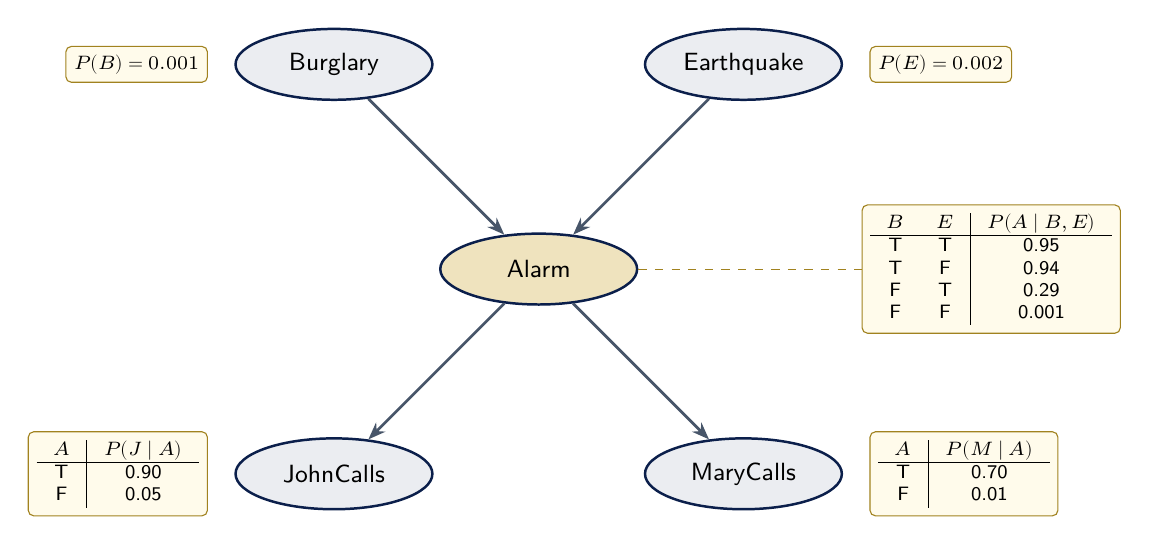
\begin{tikzpicture}[x=1cm,y=1cm,rv/.style={ellipse,draw=navy,fill=navy!8,line width=0.9pt,font=\sffamily\small,minimum width=25mm,minimum height=9mm},
  cpt/.style={font=\sffamily\scriptsize,draw=gold!80!black,fill=outbg,rounded corners=2pt,inner sep=3pt}]
  \node[rv] (B) at (-2.6,0) {Burglary}; \node[rv] (E) at (2.6,0) {Earthquake};
  \node[rv,fill=gold!30] (A) at (0,-2.6) {Alarm};
  \node[rv] (J) at (-2.6,-5.2) {JohnCalls}; \node[rv] (M) at (2.6,-5.2) {MaryCalls};
  \draw[arr,line width=1pt] (B) -- (A); \draw[arr,line width=1pt] (E) -- (A); \draw[arr,line width=1pt] (A) -- (J); \draw[arr,line width=1pt] (A) -- (M);
  \node[cpt,anchor=east] at (-4.2,0) {$P(B)=0.001$};
  \node[cpt,anchor=west] at (4.2,0) {$P(E)=0.002$};
  \node[cpt,anchor=west] at (4.1,-2.6) {\begin{tabular}{cc|c} $B$ & $E$ & $P(A\mid B,E)$\\ \hline T & T & 0.95\\ T & F & 0.94\\ F & T & 0.29\\ F & F & 0.001\end{tabular}};
  \draw[dashed,gold!80!black] (A.east) -- (4.1,-2.6);
  \node[cpt,anchor=east] at (-4.2,-5.2) {\begin{tabular}{c|c} $A$ & $P(J\mid A)$\\ \hline T & 0.90\\ F & 0.05\end{tabular}};
  \node[cpt,anchor=west] at (4.2,-5.2) {\begin{tabular}{c|c} $A$ & $P(M\mid A)$\\ \hline T & 0.70\\ F & 0.01\end{tabular}};
\end{tikzpicture}
\end{diagram}

\begin{example}
A disease affects 1\% of people. A test detects it in 95\% of patients (sensitivity) and is wrongly positive for 5\% of healthy people. Out of 10,000 people:
\begin{itemize}
  \item 100 have the disease $\Rightarrow$ 95 test positive;
  \item 9,900 are healthy $\Rightarrow$ 495 test positive.
\end{itemize}
So among the $95+495=590$ positive results only 95 are true: $P(D\mid +)=95/590\approx 0.161$. A positive test raises the belief from 1\% to about 16\%, not to 95\%.
\end{example}

\begin{maths}
\textbf{Bayes' theorem} with the law of total probability in the denominator:
\[ P(D\mid +)=\frac{P(+\mid D)\,P(D)}{P(+\mid D)\,P(D)+P(+\mid\lnot D)\,P(\lnot D)}
=\frac{0.95\times0.01}{0.95\times0.01+0.05\times0.99}=\frac{0.0095}{0.0590}=0.161 . \]
\textbf{Bayesian network semantics} (chain rule over parents):
\begin{align*}
P(x_1,\dots,x_n)&=\prod_{i=1}^{n}P\bigl(x_i\mid \mathrm{Parents}(X_i)\bigr),\\
P(B,E,A,J,M)&=P(B)\,P(E)\,P(A\mid B,E)\,P(J\mid A)\,P(M\mid A).
\end{align*}
The network needs only $1+1+4+2+2=10$ numbers instead of $2^{5}-1=31$ for the full joint table.

\textbf{Inference by enumeration} for query $X$, evidence $\mathbf{e}$ and hidden variables $\mathbf{y}$:
\begin{align*}
P(X\mid \mathbf{e})&=\alpha\sum_{\mathbf{y}}P(X,\mathbf{e},\mathbf{y}),\\
P(B\mid j,m)&=\alpha\,P(B)\sum_{e}P(e)\sum_{a}P(a\mid B,e)\,P(j\mid a)\,P(m\mid a).
\end{align*}
Evaluating gives $P(b\mid j,m)=\alpha\times 0.00059224$ and $P(\lnot b\mid j,m)=\alpha\times 0.0014919$, hence
\[ P(b\mid j,m)=\frac{0.00059224}{0.00059224+0.0014919}\approx 0.284 . \]
\end{maths}

\begin{algorithm}
\begin{enumerate}
  \item Store the prior probabilities and the CPT of every node.
  \item Write a function \texttt{joint} that multiplies $P(\text{node}\mid\text{parents})$ over all five nodes.
  \item For a query, enumerate all $2^{5}=32$ truth assignments; keep those that agree with the evidence.
  \item Add the joint probability of each kept assignment to the total for the query variable being true or false.
  \item Normalise: divide the ``true'' total by the sum of both totals.
\end{enumerate}
\end{algorithm}

\begin{pycode}{exp08\_bayes\_network.py}
"""Experiment 8: Bayes' theorem and a Bayesian network for diagnosis."""
from itertools import product


# ---------------- Part A: Bayes' theorem (medical test) ----------------
def bayes(prior, sensitivity, false_positive_rate):
    """P(Disease | Positive test)."""
    evidence = sensitivity * prior + false_positive_rate * (1 - prior)
    return sensitivity * prior / evidence, evidence


# ---------------- Part B: Burglary-alarm Bayesian network ----------------
#        Burglary     Earthquake
#              \       /
#                Alarm
#              /       \
#      JohnCalls     MaryCalls
VARS = ["B", "E", "A", "J", "M"]
P_B = 0.001
P_E = 0.002
P_A = {(True, True): 0.95, (True, False): 0.94,
       (False, True): 0.29, (False, False): 0.001}      # P(A=T | B, E)
P_J = {True: 0.90, False: 0.05}                         # P(J=T | A)
P_M = {True: 0.70, False: 0.01}                         # P(M=T | A)


def pr(p_true, value):
    return p_true if value else 1 - p_true


def joint(b, e, a, j, m):
    """Chain rule for the network: product of P(node | parents)."""
    return (pr(P_B, b) * pr(P_E, e) * pr(P_A[(b, e)], a)
            * pr(P_J[a], j) * pr(P_M[a], m))


def query(var, evidence):
    """Inference by enumeration: P(var = True | evidence)."""
    dist = {True: 0.0, False: 0.0}
    for values in product([True, False], repeat=len(VARS)):
        world = dict(zip(VARS, values))
        if all(world[k] == v for k, v in evidence.items()):
            dist[world[var]] += joint(*values)
    return dist[True] / (dist[True] + dist[False])


if __name__ == "__main__":
    print("PART A: Bayes' theorem for a diagnostic test")
    prior, sens, fpr = 0.01, 0.95, 0.05
    print(f"   P(D) = {prior}, P(+|D) = {sens}, P(+|~D) = {fpr}")
    post, evidence = bayes(prior, sens, fpr)
    print(f"   P(+)    = {evidence:.4f}")
    print(f"   P(D|+)  = {post:.4f}")
    post2, _ = bayes(post, sens, fpr)
    print(f"   P(D|++) = {post2:.4f}   (second independent positive test)")

    print("\nPART B: Burglary network, inference by enumeration")
    print(f"   P(J=T, M=T, A=T, B=F, E=F) = "
          f"{joint(False, False, True, True, True):.6f}")
    tests = [
        ("B", {}),
        ("A", {}),
        ("B", {"A": True}),
        ("B", {"J": True}),
        ("B", {"J": True, "M": True}),
        ("E", {"J": True, "M": True}),
        ("A", {"J": True, "M": True}),
        ("B", {"J": True, "M": True, "E": True}),
    ]
    for var, ev in tests:
        given = ", ".join(f"{k}={'T' if v else 'F'}" for k, v in ev.items())
        label = f"P({var}=T | {given})" if given else f"P({var}=T)"
        print(f"   {label:<26} = {query(var, ev):.4f}")
\end{pycode}

\begin{inputbox}
Part A: prior $P(D)=0.01$, sensitivity $P(+\mid D)=0.95$, false-positive rate $P(+\mid\lnot D)=0.05$. Part B: the CPT values shown in the diagram and eight queries given as (variable, evidence) pairs in the list \texttt{tests}.
\end{inputbox}

\begin{outputbox}
PART A: Bayes' theorem for a diagnostic test
   P(D) = 0.01, P(+|D) = 0.95, P(+|~D) = 0.05
   P(+)    = 0.0590
   P(D|+)  = 0.1610
   P(D|++) = 0.7848   (second independent positive test)

PART B: Burglary network, inference by enumeration
   P(J=T, M=T, A=T, B=F, E=F) = 0.000628
   P(B=T)                     = 0.0010
   P(A=T)                     = 0.0025
   P(B=T | A=T)               = 0.3736
   P(B=T | J=T)               = 0.0163
   P(B=T | J=T, M=T)          = 0.2842
   P(E=T | J=T, M=T)          = 0.1761
   P(A=T | J=T, M=T)          = 0.7607
   P(B=T | J=T, M=T, E=T)     = 0.0033
\end{outputbox}

\begin{result}
Bayes' theorem gave $P(D\mid +)=0.161$. For the Bayesian network, $P(\mathit{Burglary}\mid \mathit{JohnCalls},\mathit{MaryCalls})=0.284$. When an earthquake is also known, the probability of burglary falls to 0.003: the earthquake ``explains away'' the alarm.
\end{result}

\begin{viva}
\begin{enumerate}
  \item State Bayes' theorem and name prior, likelihood, evidence and posterior.
  \item Why is $P(D\mid +)$ so small even though the test is 95\% accurate?
  \item What conditional independence does the burglary network assume about John and Mary?
  \item What is meant by ``explaining away''?
  \item Why is inference by enumeration impractical for large networks?
\end{enumerate}
\end{viva}

% ============================ EXPERIMENT 9 ===========================
\experiment{Building a Decision-Tree Classifier on a Small Dataset and Interpreting the Rules Learned}{CO204.5}{Decision-Tree Classifier}

\begin{aim}
To build a decision-tree classifier using the ID3 algorithm (entropy and information gain) on the Play-Tennis dataset and to interpret the IF--THEN rules it learns.
\end{aim}

\begin{descr}
A decision tree is a supervised learning model. Each internal node tests an attribute, each branch is a value of that attribute and each leaf is a class label. \textbf{ID3} builds the tree top-down: at each node it chooses the attribute that gives the largest \emph{information gain}, i.e. the largest reduction in entropy (impurity) of the class labels, splits the data, and repeats on each subset until the subset is pure. Every root-to-leaf path can be read as a human-understandable rule, which makes decision trees an \emph{interpretable} model.
\end{descr}

\begin{inputbox}
The Play-Tennis dataset (14 examples, 4 attributes, class \textit{PlayTennis}) and one unseen day to classify.
\begin{center}\sffamily\footnotesize
\rowcolors{2}{orange!7}{white}
\begin{tabular}{clllll@{\hskip 6mm}clllll}
\rowcolor{orange!30} Day & Outlook & Temp. & Humidity & Wind & Play & Day & Outlook & Temp. & Humidity & Wind & Play\\
1 & Sunny & Hot & High & Weak & No & 8 & Sunny & Mild & High & Weak & No\\
2 & Sunny & Hot & High & Strong & No & 9 & Sunny & Cool & Normal & Weak & Yes\\
3 & Overcast & Hot & High & Weak & Yes & 10 & Rain & Mild & Normal & Weak & Yes\\
4 & Rain & Mild & High & Weak & Yes & 11 & Sunny & Mild & Normal & Strong & Yes\\
5 & Rain & Cool & Normal & Weak & Yes & 12 & Overcast & Mild & High & Strong & Yes\\
6 & Rain & Cool & Normal & Strong & No & 13 & Overcast & Hot & Normal & Weak & Yes\\
7 & Overcast & Cool & Normal & Strong & Yes & 14 & Rain & Mild & High & Strong & No\\
\end{tabular}
\end{center}
\end{inputbox}

\begin{diagram}{the decision tree learned by ID3}
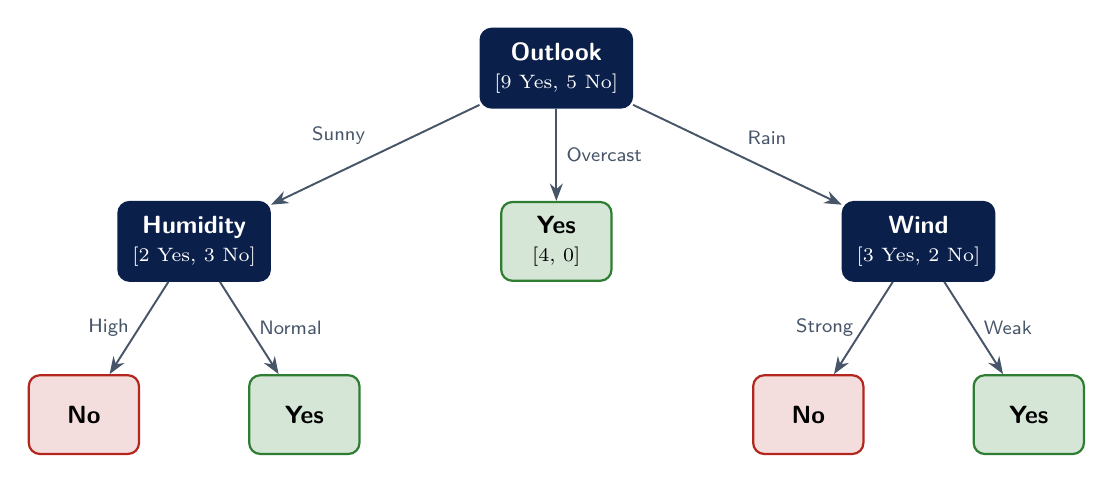
\begin{tikzpicture}[x=1cm,y=1cm,
  dn/.style={blk,fill=navy,text=white,font=\sffamily\bfseries\small},
  yes/.style={blk,fill=dgreen!20,draw=dgreen,font=\sffamily\bfseries\small,minimum width=14mm},
  no/.style={blk,fill=crimson!15,draw=crimson,font=\sffamily\bfseries\small,minimum width=14mm}]
  \node[dn] (o) at (0,0) {Outlook\\[-1pt]{\normalfont\scriptsize [9 Yes, 5 No]}};
  \node[dn] (h) at (-4.6,-2.2) {Humidity\\[-1pt]{\normalfont\scriptsize [2 Yes, 3 No]}};
  \node[yes] (y0) at (0,-2.2) {Yes\\[-1pt]{\normalfont\scriptsize [4, 0]}};
  \node[dn] (w) at (4.6,-2.2) {Wind\\[-1pt]{\normalfont\scriptsize [3 Yes, 2 No]}};
  \node[no] (n1) at (-6.0,-4.4) {No}; \node[yes] (y1) at (-3.2,-4.4) {Yes};
  \node[no] (n2) at (3.2,-4.4) {No}; \node[yes] (y2) at (6.0,-4.4) {Yes};
  \draw[arr] (o) -- node[lbl,above left]{Sunny} (h); \draw[arr] (o) -- node[lbl,right]{Overcast} (y0); \draw[arr] (o) -- node[lbl,above right]{Rain} (w);
  \draw[arr] (h) -- node[lbl,left]{High} (n1); \draw[arr] (h) -- node[lbl,right]{Normal} (y1);
  \draw[arr] (w) -- node[lbl,left]{Strong} (n2); \draw[arr] (w) -- node[lbl,right]{Weak} (y2);
\end{tikzpicture}
\end{diagram}

\begin{example}
\textbf{Choosing the root.} The full set $S$ has 9 Yes and 5 No. Splitting on \textit{Outlook} gives Sunny [2 Yes, 3 No], Overcast [4 Yes, 0 No], Rain [3 Yes, 2 No]. The \textit{Overcast} branch is already pure, so \textit{Outlook} removes much uncertainty. The calculation in the next box gives Gain = 0.247, the largest of the four attributes, so \textit{Outlook} becomes the root.
\end{example}

\begin{maths}
\textbf{Entropy} of a set $S$ with class proportions $p_c$:\qquad $H(S)=-\sum_{c}p_c\log_2 p_c$.
\[ H(S)=-\tfrac{9}{14}\log_2\tfrac{9}{14}-\tfrac{5}{14}\log_2\tfrac{5}{14}=0.940\ \text{bits}. \]
\textbf{Information gain} of attribute $A$:\qquad $\displaystyle \mathrm{Gain}(S,A)=H(S)-\sum_{v\in \mathrm{Values}(A)}\frac{|S_v|}{|S|}\,H(S_v)$.

For \textit{Outlook}: $H(S_{\text{Sunny}})=H(S_{\text{Rain}})=-\tfrac25\log_2\tfrac25-\tfrac35\log_2\tfrac35=0.971$ and $H(S_{\text{Overcast}})=0$, so
\[ \mathrm{Gain}(S,\textit{Outlook})=0.940-\Bigl[\tfrac{5}{14}(0.971)+\tfrac{4}{14}(0)+\tfrac{5}{14}(0.971)\Bigr]=0.940-0.694=0.247 . \]
Similarly $\mathrm{Gain}(S,\textit{Humidity})=0.152$, $\mathrm{Gain}(S,\textit{Wind})=0.048$, $\mathrm{Gain}(S,\textit{Temperature})=0.029$.

\textbf{Alternative impurity measure (CART):}\quad $\mathrm{Gini}(S)=1-\sum_c p_c^{2}$.
\end{maths}

\begin{algorithm}
\textbf{ID3(examples, attributes)}
\begin{enumerate}
  \item If all examples have the same class, return a leaf with that class.
  \item If no attribute is left, return a leaf with the majority class.
  \item Compute the information gain of every remaining attribute and choose the best one, $A$.
  \item Create a node that tests $A$; for each value $v$ of $A$ call ID3 on the examples with $A=v$ and the remaining attributes.
  \item Read each root-to-leaf path as a rule: IF (tests on the path) THEN class.
\end{enumerate}
\end{algorithm}

\begin{pycode}{exp09\_decision\_tree\_id3.py}
"""Experiment 9: Decision-tree classifier (ID3) on the Play-Tennis dataset."""
from collections import Counter
from math import log2

ATTRIBUTES = ["Outlook", "Temperature", "Humidity", "Wind"]
DATA = [  # Outlook, Temperature, Humidity, Wind, PlayTennis
    ("Sunny", "Hot", "High", "Weak", "No"),
    ("Sunny", "Hot", "High", "Strong", "No"),
    ("Overcast", "Hot", "High", "Weak", "Yes"),
    ("Rain", "Mild", "High", "Weak", "Yes"),
    ("Rain", "Cool", "Normal", "Weak", "Yes"),
    ("Rain", "Cool", "Normal", "Strong", "No"),
    ("Overcast", "Cool", "Normal", "Strong", "Yes"),
    ("Sunny", "Mild", "High", "Weak", "No"),
    ("Sunny", "Cool", "Normal", "Weak", "Yes"),
    ("Rain", "Mild", "Normal", "Weak", "Yes"),
    ("Sunny", "Mild", "Normal", "Strong", "Yes"),
    ("Overcast", "Mild", "High", "Strong", "Yes"),
    ("Overcast", "Hot", "Normal", "Weak", "Yes"),
    ("Rain", "Mild", "High", "Strong", "No"),
]


def entropy(rows):
    counts = Counter(r[-1] for r in rows)
    return -sum(c / len(rows) * log2(c / len(rows)) for c in counts.values())


def information_gain(rows, col):
    remainder = 0.0
    for value in set(r[col] for r in rows):
        subset = [r for r in rows if r[col] == value]
        remainder += len(subset) / len(rows) * entropy(subset)
    return entropy(rows) - remainder


def id3(rows, columns, depth=0):
    """Return a leaf label or a node {attribute: {value: subtree}}."""
    labels = [r[-1] for r in rows]
    if len(set(labels)) == 1:                  # pure node
        return labels[0]
    if not columns:                            # no attribute left
        return Counter(labels).most_common(1)[0][0]
    gains = {c: information_gain(rows, c) for c in columns}
    best = max(columns, key=lambda c: gains[c])
    if depth == 0:
        print("Information gain at the root:")
        for c in columns:
            print(f"   Gain(S, {ATTRIBUTES[c]:<11}) = {gains[c]:.4f}")
        print(f"   => split on {ATTRIBUTES[best]}\n")
    node = {ATTRIBUTES[best]: {}}
    for value in sorted(set(r[best] for r in rows)):
        subset = [r for r in rows if r[best] == value]
        remaining = [c for c in columns if c != best]
        node[ATTRIBUTES[best]][value] = id3(subset, remaining, depth + 1)
    return node


def show_tree(node, indent="   "):
    if not isinstance(node, dict):
        print(f"{indent}-> {node}")
        return
    (attribute, branches), = node.items()
    for value, child in branches.items():
        print(f"{indent}[{attribute} = {value}]")
        show_tree(child, indent + "    ")


def extract_rules(node, conditions=()):
    if not isinstance(node, dict):
        yield conditions, node
        return
    (attribute, branches), = node.items()
    for value, child in branches.items():
        yield from extract_rules(child, conditions + ((attribute, value),))


def predict(node, sample):
    while isinstance(node, dict):
        (attribute, branches), = node.items()
        node = branches[sample[attribute]]
    return node


if __name__ == "__main__":
    print(f"Training examples: {len(DATA)}   "
          f"Entropy(S) = {entropy(DATA):.4f}\n")
    tree = id3(DATA, list(range(len(ATTRIBUTES))))
    print("Decision tree learned:")
    show_tree(tree)

    print("\nRules read from the tree:")
    for i, (conds, label) in enumerate(extract_rules(tree), 1):
        lhs = " AND ".join(f"{a} = {v}" for a, v in conds)
        print(f"   R{i}: IF {lhs} THEN PlayTennis = {label}")

    correct = sum(predict(tree, dict(zip(ATTRIBUTES, r))) == r[-1] for r in DATA)
    print(f"\nTraining accuracy: {correct}/{len(DATA)}")
    new_day = {"Outlook": "Sunny", "Temperature": "Cool",
               "Humidity": "High", "Wind": "Strong"}
    print("New sample :", new_day)
    print("Prediction : PlayTennis =", predict(tree, new_day))
\end{pycode}

\begin{outputbox}
Training examples: 14   Entropy(S) = 0.9403

Information gain at the root:
   Gain(S, Outlook    ) = 0.2467
   Gain(S, Temperature) = 0.0292
   Gain(S, Humidity   ) = 0.1518
   Gain(S, Wind       ) = 0.0481
   => split on Outlook

Decision tree learned:
   [Outlook = Overcast]
       -> Yes
   [Outlook = Rain]
       [Wind = Strong]
           -> No
       [Wind = Weak]
           -> Yes
   [Outlook = Sunny]
       [Humidity = High]
           -> No
       [Humidity = Normal]
           -> Yes

Rules read from the tree:
   R1: IF Outlook = Overcast THEN PlayTennis = Yes
   R2: IF Outlook = Rain AND Wind = Strong THEN PlayTennis = No
   R3: IF Outlook = Rain AND Wind = Weak THEN PlayTennis = Yes
   R4: IF Outlook = Sunny AND Humidity = High THEN PlayTennis = No
   R5: IF Outlook = Sunny AND Humidity = Normal THEN PlayTennis = Yes

Training accuracy: 14/14
New sample : {'Outlook': 'Sunny', 'Temperature': 'Cool', 'Humidity': 'High', 'Wind': 'Strong'}
Prediction : PlayTennis = No
\end{outputbox}

\begin{result}
ID3 selected \textit{Outlook} as the root (gain 0.247) and learned a tree with five leaves that classifies all 14 training examples correctly. The tree yields five readable rules; \textit{Temperature} was never used, showing that it is not needed to decide the class in this dataset.
\end{result}

\begin{viva}
\begin{enumerate}
  \item What does an entropy of 0 mean? What does an entropy of 1 mean for two classes?
  \item Why does ID3 prefer the attribute with the highest information gain?
  \item What is overfitting in decision trees and how does pruning help?
  \item How do C4.5 and CART differ from ID3?
  \item Is 100\% training accuracy a guarantee of good performance on new data? Why?
\end{enumerate}
\end{viva}

% ============================ EXPERIMENT 10 ==========================
\experiment{Mini-Project: A Simple Rule-Based Expert System and a Basic Chatbot}{CO204.5}{Expert System / Chatbot}

\begin{aim}
To develop (a) a rule-based expert system that identifies an animal from observed features using forward chaining with an explanation facility, and (b) a basic pattern-matching chatbot.
\end{aim}

\begin{descr}
An \textbf{expert system} imitates the decision-making of a human expert in a narrow domain. Its knowledge is kept \emph{separate} from the reasoning program: the \textbf{knowledge base} holds IF--THEN production rules, the \textbf{working memory} holds the facts of the current case, and the \textbf{inference engine} fires rules whose conditions are satisfied. An \textbf{explanation facility} reports which rules fired, so the user can see \emph{how} the conclusion was reached.

A \textbf{rule-based chatbot} (in the style of ELIZA) matches the user's sentence against a list of patterns and replies with the response attached to the first pattern that matches. Both systems are examples of symbolic AI driven by hand-written rules.
\end{descr}

\begin{diagram}{architecture of the expert system and the chatbot pipeline}
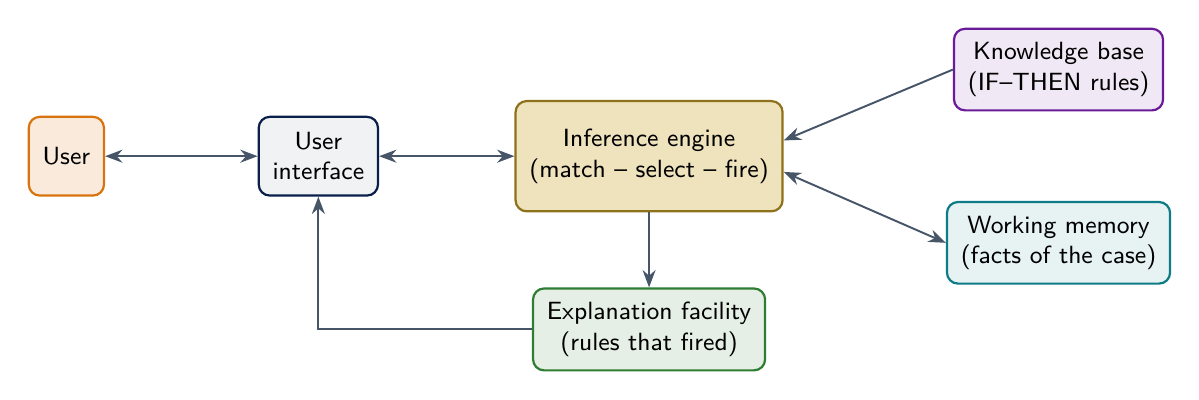
\begin{tikzpicture}[x=1cm,y=1cm]
  \node[blk,fill=orange!15,draw=orange] (u) at (0,0) {User};
  \node[blk] (ui) at (3.2,0) {User\\ interface};
  \node[blk,fill=gold!30,draw=gold!70!black,minimum height=14mm] (ie) at (7.4,0) {Inference engine\\ (match -- select -- fire)};
  \node[blk,fill=purple!10,draw=purple] (kb) at (12.6,1.1) {Knowledge base\\ (IF--THEN rules)};
  \node[blk,fill=teal!10,draw=teal] (wm) at (12.6,-1.1) {Working memory\\ (facts of the case)};
  \node[blk,fill=dgreen!12,draw=dgreen] (ex) at (7.4,-2.2) {Explanation facility\\ (rules that fired)};
  \draw[arr,{Stealth[length=2.2mm]}-{Stealth[length=2.2mm]}] (u) -- (ui);
  \draw[arr,{Stealth[length=2.2mm]}-{Stealth[length=2.2mm]}] (ui) -- (ie);
  \draw[arr] (kb.west) -- ([yshift=2mm]ie.east);
  \draw[arr,{Stealth[length=2.2mm]}-{Stealth[length=2.2mm]}] (wm.west) -- ([yshift=-2mm]ie.east);
  \draw[arr] (ie) -- (ex); \draw[arr] (ex.west) -| (ui.south);
\end{tikzpicture}

\vspace{6pt}
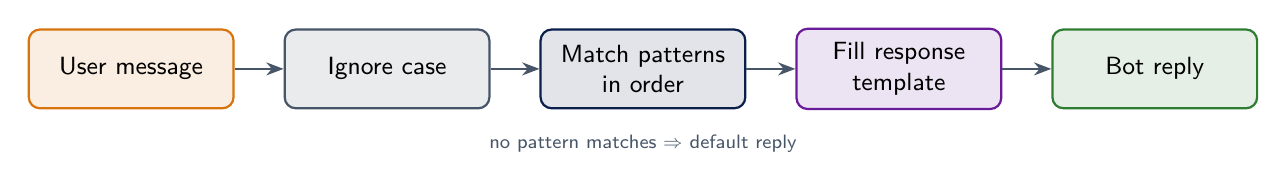
\begin{tikzpicture}[x=1cm,y=1cm]
  \foreach \t/\col [count=\i from 0] in {User message/orange,Ignore case/slate,Match patterns\\ in order/navy,Fill response\\ template/purple,Bot reply/dgreen}{
    \node[blk,fill=\col!12,draw=\col,minimum width=26mm] (c\i) at (\i*3.25,0) {\t};}
  \foreach \i/\j in {0/1,1/2,2/3,3/4} \draw[arr] (c\i) -- (c\j);
  \node[lbl] at (6.5,-0.95) {no pattern matches $\Rightarrow$ default reply};
\end{tikzpicture}
\end{diagram}

\begin{example}
Observed facts: \{has hair, eats meat, has tawny colour, has black stripes\}.
\begin{enumerate}
  \item R1: has hair $\Rightarrow$ \textit{is a mammal} (added to working memory).
  \item R5: is a mammal AND eats meat $\Rightarrow$ \textit{is a carnivore}.
  \item R8: is a carnivore AND has tawny colour AND has black stripes $\Rightarrow$ \textit{is a TIGER}.
\end{enumerate}
No further rule can fire, so the system reports TIGER together with the chain R1, R5, R8 as its explanation.
\end{example}

\begin{maths}
\textbf{Production rule:}\quad $R_k:\; c_1\land c_2\land\dots\land c_m \Rightarrow a$.\quad With working memory $W$, rule $R_k$ is \emph{applicable} when $\{c_1,\dots,c_m\}\subseteq W$ (in the program: \texttt{conditions <= memory}).

\textbf{Forward chaining (data-driven):}
\[ W_0=\text{observations},\qquad W_{t+1}=W_t\cup\{\,a \mid (C\Rightarrow a)\in KB,\ C\subseteq W_t\,\},\qquad \text{stop when } W_{t+1}=W_t . \]
Since $W$ only grows and the number of possible conclusions is finite, the loop terminates; with $r$ rules it needs at most $r$ passes, i.e. $O(r^{2})$ rule checks.

\textbf{Recognise--act cycle:} match (find applicable rules, the conflict set) $\to$ select (conflict resolution, here rule order) $\to$ act (add the conclusion).

\textbf{Uncertain rules (MYCIN certainty factors),} for further study: when two rules support the same conclusion with $CF_1, CF_2 > 0$,
$\;CF = CF_1 + CF_2\,(1-CF_1)$.

\textbf{Chatbot:} the reply is $\mathrm{resp}(p_i)$ for the smallest index $i$ such that the regular expression $p_i$ matches the message $m$; captured groups of $p_i$ are substituted into the template.
\end{maths}

\begin{algorithm}
\textbf{Expert system}
\begin{enumerate}
  \item Load the observed facts into working memory.
  \item Scan the rules; if all conditions of a rule are in working memory and its conclusion is not, add the conclusion and record the rule.
  \item Repeat step 2 until a full scan adds nothing.
  \item Report the identified animal and the recorded rules as the explanation.
\end{enumerate}
\textbf{Chatbot}
\begin{enumerate}
  \item Read the user's message.
  \item Test the patterns in order, ignoring case; on the first match, fill the response template with the captured words.
  \item If nothing matches, give the default reply.
\end{enumerate}
\end{algorithm}

\begin{pycode}{exp10\_expert\_system\_chatbot.py}
"""Experiment 10 (Mini-project): Rule-based expert system and a basic chatbot.
Part A: animal-identification expert system (forward chaining + explanation).
Part B: pattern-matching helpdesk chatbot."""
import re

# ---------------- Part A: expert system ----------------
RULES = [  # (rule id, IF all of these facts, THEN conclude this fact)
    ("R1", {"has hair"}, "is a mammal"),
    ("R2", {"gives milk"}, "is a mammal"),
    ("R3", {"has feathers"}, "is a bird"),
    ("R4", {"flies", "lays eggs"}, "is a bird"),
    ("R5", {"is a mammal", "eats meat"}, "is a carnivore"),
    ("R6", {"is a mammal", "has hooves"}, "is an ungulate"),
    ("R7", {"is a carnivore", "has tawny colour", "has dark spots"},
     "is a CHEETAH"),
    ("R8", {"is a carnivore", "has tawny colour", "has black stripes"},
     "is a TIGER"),
    ("R9", {"is an ungulate", "has long neck", "has dark spots"},
     "is a GIRAFFE"),
    ("R10", {"is an ungulate", "has black stripes"}, "is a ZEBRA"),
    ("R11", {"is a bird", "cannot fly", "swims"}, "is a PENGUIN"),
    ("R12", {"is a bird", "flies well"}, "is an ALBATROSS"),
]


def infer(observations):
    """Forward chaining: fire rules until working memory stops growing."""
    memory, fired = set(observations), []
    changed = True
    while changed:
        changed = False
        for rule_id, conditions, conclusion in RULES:
            if conditions <= memory and conclusion not in memory:
                memory.add(conclusion)
                fired.append((rule_id, conditions, conclusion))
                changed = True
    return memory, fired


def consult(name, observations):
    print(f"Case: {name}")
    print("   Observed :", ", ".join(sorted(observations)))
    memory, fired = infer(observations)
    for rule_id, conditions, conclusion in fired:       # explanation facility
        print(f"   {rule_id:<3} fired: {' AND '.join(sorted(conditions))} "
              f"=> {conclusion}")
    verdict = [f for f in memory if f.split()[-1].isupper()]
    print("   Diagnosis:", verdict[0] if verdict else "animal not identified")


# ---------------- Part B: chatbot ----------------
PATTERNS = [
    (r"\b(hi|hello|hey|namaste)\b",
     "Hello! I am AI-Lab Bot. Ask me about the AI laboratory."),
    (r"\bmy name is (\w+)", "Nice to meet you, {0}!"),
    (r"\b(timing|time|when)\b",
     "The AI lab runs for 2 hours every week as per your batch timetable."),
    (r"\b(experiments?|practicals?)\b",
     "There are 10 experiments: search, games, CSP, logic, Bayes, "
     "decision trees and a mini-project."),
    (r"\b(language|python|prolog)\b",
     "We use Python 3. Experiment 6 may also be done in Prolog."),
    (r"\b(book|textbook|reference)\b",
     "Refer to Russell and Norvig, 'Artificial Intelligence: A Modern "
     "Approach'."),
    (r"\bi am (stuck|confused|lost)\b",
     "Do not worry about being {0}. Trace the algorithm by hand first."),
    (r"\b(thanks|thank you)\b", "You are welcome. Happy learning!"),
    (r"\b(bye|exit|quit)\b", "Goodbye!"),
]
DEFAULT = "Sorry, I did not understand. Try asking about experiments or timing."


def reply(message):
    for pattern, answer in PATTERNS:
        found = re.search(pattern, message, re.IGNORECASE)
        if found:
            return answer.format(*found.groups())
    return DEFAULT


if __name__ == "__main__":
    print("PART A: Animal identification expert system")
    consult("Animal 1", {"has hair", "eats meat", "has tawny colour",
                         "has black stripes"})
    consult("Animal 2", {"has feathers", "cannot fly", "swims"})
    consult("Animal 3", {"gives milk", "has hooves", "has long neck",
                         "has dark spots"})
    consult("Animal 4", {"has scales", "swims"})

    print("\nPART B: Chatbot session")
    for message in ["Hello", "My name is Asha", "How many experiments are there?",
                    "Which language do we use?", "I am stuck in A* search",
                    "What is the weather today?", "Thanks, bye"]:
        print("   You :", message)
        print("   Bot :", reply(message))
\end{pycode}

\begin{inputbox}
Part A: four cases, each a set of observed features (the fourth cannot be identified with the given rules). Part B: seven user messages. To make either part interactive, replace the fixed lists with \texttt{input()} inside a loop.
\end{inputbox}

\begin{outputbox}
PART A: Animal identification expert system
Case: Animal 1
   Observed : eats meat, has black stripes, has hair, has tawny colour
   R1  fired: has hair => is a mammal
   R5  fired: eats meat AND is a mammal => is a carnivore
   R8  fired: has black stripes AND has tawny colour AND is a carnivore => is a TIGER
   Diagnosis: is a TIGER
Case: Animal 2
   Observed : cannot fly, has feathers, swims
   R3  fired: has feathers => is a bird
   R11 fired: cannot fly AND is a bird AND swims => is a PENGUIN
   Diagnosis: is a PENGUIN
Case: Animal 3
   Observed : gives milk, has dark spots, has hooves, has long neck
   R2  fired: gives milk => is a mammal
   R6  fired: has hooves AND is a mammal => is an ungulate
   R9  fired: has dark spots AND has long neck AND is an ungulate => is a GIRAFFE
   Diagnosis: is a GIRAFFE
Case: Animal 4
   Observed : has scales, swims
   Diagnosis: animal not identified

PART B: Chatbot session
   You : Hello
   Bot : Hello! I am AI-Lab Bot. Ask me about the AI laboratory.
   You : My name is Asha
   Bot : Nice to meet you, Asha!
   You : How many experiments are there?
   Bot : There are 10 experiments: search, games, CSP, logic, Bayes, decision trees and a mini-project.
   You : Which language do we use?
   Bot : We use Python 3. Experiment 6 may also be done in Prolog.
   You : I am stuck in A* search
   Bot : Do not worry about being stuck. Trace the algorithm by hand first.
   You : What is the weather today?
   Bot : Sorry, I did not understand. Try asking about experiments or timing.
   You : Thanks, bye
   Bot : You are welcome. Happy learning!
\end{outputbox}

\begin{result}
The expert system identified the tiger, penguin and giraffe by chaining rules, explained every conclusion, and honestly reported when its knowledge was insufficient. The chatbot answered the scripted questions using pattern matching and fell back to a default reply for an unknown question.
\end{result}

\begin{secbox}{MINI-PROJECT EXTENSIONS}{teal}
\begin{enumerate}
  \item Add at least eight new rules (for example for ostrich, eagle or dolphin) and test them.
  \item Add a \emph{why} facility: let the system ask the user for a missing fact and state which rule needs it (backward chaining).
  \item Attach certainty factors to rules and report the confidence of the conclusion.
  \item Extend the chatbot with a memory of the user's name and with at least ten new patterns for your department helpdesk.
  \item Discuss one ethical issue of chatbots (for example privacy of user messages or over-trust in automated advice).
\end{enumerate}
\end{secbox}

\begin{viva}
\begin{enumerate}
  \item Name the main components of an expert system.
  \item Why is the knowledge base kept separate from the inference engine?
  \item What is conflict resolution? Name two strategies.
  \item Compare forward chaining with backward chaining for diagnosis problems.
  \item What are the limitations of rule-based chatbots compared with learning-based ones?
\end{enumerate}
\end{viva}

% ============================ REFERENCES =============================
\clearpage
\markright{Learning Resources}
{\sffamily\bfseries\Large\color{navy}Learning Resources}\par
{\color{gold}\rule{\textwidth}{1.2pt}}

\begin{secbox}{TEXT BOOKS}{navy}
\begin{enumerate}
  \item Russell, S., \& Norvig, P. (2021). \textit{Artificial Intelligence: A Modern Approach} (4th ed.). Pearson. ISBN: 978-0134610993.
  \item Rich, E., Knight, K., \& Nair, S. B. (2017). \textit{Artificial Intelligence} (3rd ed.). McGraw Hill Education. ISBN: 978-0070087705.
\end{enumerate}
\end{secbox}
\begin{secbox}{REFERENCE BOOKS}{teal}
\begin{enumerate}
  \item Luger, G. F. (2008). \textit{Artificial Intelligence: Structures and Strategies for Complex Problem Solving} (6th ed.). Pearson. ISBN: 978-0321545893.
  \item Nilsson, N. J. (1998). \textit{Artificial Intelligence: A New Synthesis}. Morgan Kaufmann. ISBN: 978-1558605350.
  \item Patterson, D. W. (2007). \textit{Introduction to Artificial Intelligence and Expert Systems}. PHI Learning. ISBN: 978-8120305779.
\end{enumerate}
\end{secbox}
\begin{secbox}{ONLINE REFERENCES}{purple}
\begin{enumerate}
  \item NPTEL: An Introduction to Artificial Intelligence, Prof. Mausam, IIT Delhi. \url{https://archive.nptel.ac.in/courses/106/102/106102220/}
  \item NPTEL: Fundamentals of Artificial Intelligence, Prof. Shyamanta M. Hazarika, IIT Guwahati. \url{https://archive.nptel.ac.in/courses/112/103/112103280/}
  \item NPTEL: Artificial Intelligence, Prof. P. Dasgupta, IIT Kharagpur. \url{https://archive.nptel.ac.in/courses/106/105/106105079/}
\end{enumerate}
\end{secbox}

\begin{secbox}{EXPERIMENT -- COURSE OUTCOME MAPPING}{gold}
\centering\sffamily\small
\renewcommand{\arraystretch}{1.25}
\begin{tabular}{l*{10}{c}}
\toprule
 & E1 & E2 & E3 & E4 & E5 & E6 & E7 & E8 & E9 & E10\\ \midrule
CO204.1 & $\checkmark$ & & & & & & & & & \\
CO204.2 & & $\checkmark$ & $\checkmark$ & $\checkmark$ & $\checkmark$ & & & & & \\
CO204.3 & & & & & & $\checkmark$ & $\checkmark$ & & & \\
CO204.4 & & & & & & & & $\checkmark$ & & \\
CO204.5 & & & & & & & & & $\checkmark$ & $\checkmark$\\
\bottomrule
\end{tabular}
\end{secbox}

\end{document}
